% LTeX: language=fr
% Copyright © 2021, Loïc Grobol <loic.grobol@gmail.com>
% This document is available under the terms of the Creative Commons Attribution 4.0 International License (CC BY 4.0) (https://creativecommons.org/licenses/by/4.0/)

\RequirePackage{xparse}
\RequirePackage{shellesc}
% Settings
\newcommand\myname{Loïc Grobol}
\newcommand\mylab{MoDyCo, Université Paris Nanterre}
\newcommand\pdftitle{Cours 4 : Arbres et analyseurs syntaxiques}
\newcommand\mymail{lgrobol@parisnanterre.fr}
\newcommand\titlepagetitle{\pdftitle}
\newcommand\eventname{Données structurées}
\newcommand\eventvenue{M2 PluriTAL}
\newcommand\eventdate{2021-12-13}

\documentclass[
	hyperref={unicode},
	xcolor={svgnames, table},
	aspectratio=169,
	french,
]{beamer}
% Colour palette from [Paul Tol's technical note](https://personal.sron.nl/~pault/data/colourschemes.pdf) v3.1
% Bright scheme
\definecolor{sronbrightblue}{RGB}{68, 119, 170}
\definecolor{sronbrightcyan}{RGB}{102, 204, 238}
\definecolor{sronbrightgreen}{RGB}{34, 136, 51}
\definecolor{sronbrightyellow}{RGB}{204, 187, 68}
\definecolor{sronbrightred}{RGB}{238, 102, 119}
\definecolor{sronbrightpurple}{RGB}{170, 51, 119}
\definecolor{sronbrightgrey}{RGB}{187, 187, 187}

\definecolor{sronmutedindigo}{RGB}{51,34,136}

% And my favourite purple
\definecolor{myfavouritepurple}{RGB}{113, 10, 186}

% Original colours names from Miryam, mapped to our palette

\colorlet{lightblue}{sronbrightblue}
\colorlet{lightgreen}{sronbrightgreen}
\colorlet{salmon}{sronbrightyellow}
\colorlet{purple}{sronbrightyellow}
\colorlet{bordeaux}{sronbrightred}
\definecolor{twitterBlue}{RGB}{0,172,237}


\usetheme[
	sectionpage=progressbar,
	subsectionpage=progressbar,
	progressbar=frametitle,
]{metropolis}
	\colorlet{accent}{sronmutedindigo}
	\setbeamercolor{frametitle}{
		use=normal text,
		bg=normal text.bg,
		fg=accent,
	}
	\setbeamercolor{alerted text}{fg=accent}
	\makeatletter
		\setlength{\metropolis@progressinheadfoot@linewidth}{0.5pt}
	\makeatother

% Left-align description lists
\defbeamertemplate{description item}{align left}{\insertdescriptionitem\hfill}
\setbeamertemplate{description item}[align left]

% Use non-standard fonts
\usepackage{fontspec}
\usefonttheme{professionalfonts}

\directlua{
	luaotfload.add_fallback(
		"emojifallback",
		{"NotoColorEmoji:mode=harf;"}
	)
}

\setsansfont{Atkinson Hyperlegible}[
	RawFeature={fallback=emojifallback},
]
\setmonofont[Scale=0.9]{Fira Mono}
\newfontfamily\fallbackfont{Deja Vu Sans}
\newfontfamily\emojifont{Noto Color Emoji}[Renderer=HarfBuzz]
\frenchspacing

% Fix missing glyphs in Fira by delegating to polyglossia/babel
\usepackage{newunicodechar}
	\newunicodechar{ }{~}   % U+202F NARROW NO-BREAK SPACE
	\newunicodechar{ }{ }   % U+2009 THIN SPACE

% Notes on left screen
% \usepackage{pgfpages}
% \setbeameroption{show notes on second screen=left}

\usepackage{polyglossia}
	\setmainlanguage{french}
	\setotherlanguage[variant=british]{english}

\usepackage{amsfonts,amssymb}
\usepackage{amsmath,amsthm}
\usepackage{mathtools}	% AMS Maths service pack
	\newtagform{brackets}{[}{]}	% Pour des lignes d'équation numérotées entre crochets
	\mathtoolsset{showonlyrefs, showmanualtags, mathic}	% affiche les tags manuels (\tag et \tag*) et corrige le kerning des maths inline dans un bloc italique voir la doc de mathtools
	\usetagform{brackets}	% Utilise le style de tags défini plus haut
\usepackage{lualatex-math}

\usepackage[math-style=french]{unicode-math}
	\setmathfont[Scale=1.3]{Libertinus Math}
\usepackage{newunicodechar}
	\newunicodechar{√}{\sqrt}
\usepackage{mleftright}

\usepackage{mismath}

\usepackage{tabularx}
\usepackage{multirow}
\usepackage{booktabs}
\usepackage{siunitx}
	\sisetup{
		detect-all,
		group-separator=\text{\,},
	}
	\DeclareSIUnit{\quantity}{\relax}
	\DeclareSIUnit{\words}{mots}
	\DeclareSIUnit{\sentences}{phrases}
	% Needed for italics and bold numbers in siunitx S-aligned columns
	\robustify\itshape
	\robustify\bfseries
\usepackage{multicol}
\usepackage{ccicons}
\usepackage{bookmark}
\usepackage{caption}
	\captionsetup{skip=1ex, labelformat=empty}
\usepackage{lua-ul}

\usepackage[
	english=american,
	french=guillemets,
	autostyle=true,
]{csquotes}
	\renewcommand{\mkbegdispquote}[2]{\itshape\let\emph\textbf}
	% Like `\foreignquote` but use the outside language's quotes not the inside's
	\NewDocumentCommand\quoteforeign{m m}{\enquote{\textlang{#1}{\textit{#2}}}}

\usepackage{tikz}
	\NewDocumentCommand{\textnode}{O{}mm}{\tikz[remember picture, baseline=(#2.base), inner sep=0pt]{\node[#1] (#2) {#3};}}
	\NewDocumentCommand{\mathnode}{O{}mm}{\tikz[remember picture, baseline=(#2.base), inner sep=0pt]{\node[#1] (#2) {\(\displaystyle #3\)};}}
	% Beamer utilities
	\tikzset{
		alt/.code args={<#1>#2#3}{%
			\alt<#1>{\pgfkeysalso{#2}}{\pgfkeysalso{#3}} % \pgfkeysalso doesn't change the path
		},
		invisible/.style={opacity=0},
		visible on/.style={alt={<#1>{}{invisible}}},
		accent on/.style={alt={<#1>{draw=accent, text=accent, thick}{draw}}},
	}

	% Misc utilities
	\tikzset{
		true scale/.style={scale=#1, every node/.style={transform shape}},
	}
	\usepackage[beamer, markings]{hf-tikz}
	\usepackage{pgfplots}
	\pgfplotsset{compat=1.18}
		% Due to pgfplots meddling with pgfkeys, we have to redefine alt here.
		\pgfplotsset{
			alt/.code args={<#1>#2#3}{%
			\alt<#1>{\pgfkeysalso{#2}}{\pgfkeysalso{#3}} % \pgfkeysalso doesn't change the path
			},
		}
		\pgfplotsset{compat=1.18}
		\pgfplotsset{colormap={SRON}{rgb255=(61,82,161) rgb255=(255,250,210) rgb255=(174,28,62)}} % chktex 36

	\usetikzlibrary{tikzmark}
	\usetikzlibrary{matrix, chains, graphs, graphdrawing}
	\usetikzlibrary{shapes, shapes.geometric}
	\usetikzlibrary{decorations.pathreplacing}
	\usetikzlibrary{positioning, calc, intersections}
	\usetikzlibrary{fit}

	% TikZ externalisation
	\usetikzlibrary{external}
	% Create the `tikzpics/` folder if it does not exist
	\ShellEscape{mkdir tikzpics}
	% Only externalise pictures on demand (to avoid messing up with metropolis theme)
	\tikzset{
		external/export=false,
		external/prefix=tikzpics/,
	}
	\tikzexternalize

\usepackage{forest}
	\useforestlibrary{linguistics}

\usepackage{tikz-dependency}

\usepackage[
	style=authoryear,
	useprefix=true,
	block=ragged,
	doi=false,
	isbn=false,
	maxbibnames=6,
	minbibnames=1,
	maxcitenames=2,
	mincitenames=1,
	uniquelist=false,
]{biblatex}
	% No small caps in french bib
	\DefineBibliographyExtras{french}{\restorecommand\mkbibnamefamily}
	\AtEveryBibitem{
		\ifentrytype{online}
		{} {
			\iffieldequalstr{howpublished}{online}
			{
				\clearfield{howpublished}
			} {
				\clearfield{urlyear}\clearfield{urlmonth}\clearfield{urlday}
			}
		}
	}
	% Fix bug with \insertbiblabel in author-date, see https://tex.stackexchange.com/questions/585635/beamer-biblatex-authoryear-causes-problem-with-insertbiblabel and https://github.com/josephwright/beamer/blob/865a19d4ec64f4c8e4935c19e162b8f4fd5aa190/base/beamerbaselocalstructure.sty#L501
	\let\insertbiblabel\relax
	\addbibresource{main.bib}
 
% Compact bibliography style
\setbeamertemplate{bibliography item}[text]

\AtEveryBibitem{
	\clearfield{series}
	\clearfield{pages}
	\clearname{editor}
}
\renewcommand*{\bibfont}{\tiny}

\usepackage{hyperxmp}	% XMP metadata

\usepackage[type={CC},modifier={by},version={4.0}]{doclicense}

\usepackage{todonotes}
\let\todox\todo
\renewcommand\todo[1]{\todox[inline]{#1}}

\title{\titlepagetitle}
\author{\myname~(\mylab)\\\href{mailto:\mymail}{<\nolinkurl{\mymail}>}}
\institute{}
\date{\eventname\\\eventvenue, \eventdate}

\titlegraphic{\ccby}

% Tikz styles
% Global
\tikzset{
	>=stealth,
	hair lines/.style={line width = 0.05pt, lightgray},
	accent on/.style={alt={<#1>{draw=accent, text=accent, thick}{draw}}},
	true scale/.style={scale=#1, every node/.style={transform shape}},
}

% Commands spécifiques
\NewDocumentCommand\shorturl{ O{https} O{://} m }{%
	\href{#1#2#3}{\nolinkurl{#3}}%
}

\DeclarePairedDelimiterX\compset[2]{\lbrace}{\rbrace}{#1\,\delimsize|\,#2}
\DeclarePairedDelimiterX\innprod[2]{\langle}{\rangle}{#1\,\delimsize|\,#2}

% Easy column vectors \vcord{a,b,c} ou \vcord[;]{a;b;c}
% Here be black magic
\ExplSyntaxOn % chktex 1
	\NewDocumentCommand{\vcord}{O{,}m}{\vector_main:nnnn{p}{\\}{#1}{#2}}
	\NewDocumentCommand{\tvcord}{O{,}m}{\vector_main:nnnn{psmall}{\\}{#1}{#2}}
	\seq_new:N\l__vector_arg_seq
	\cs_new_protected:Npn\vector_main:nnnn #1 #2 #3 #4{
		\seq_set_split:Nnn\l__vector_arg_seq{#3}{#4}
		\begin{#1matrix}
			\seq_use:Nnnn\l__vector_arg_seq{#2}{#2}{#2}
		\end{#1matrix}
	}
\ExplSyntaxOff % chktex 1

\NewDocumentCommand\itpause{}{%
	\addtocounter{beamerpauses}{-1}%
	\pause%
}


% ██████   ██████   ██████ ██    ██ ███    ███ ███████ ███    ██ ████████
% ██   ██ ██    ██ ██      ██    ██ ████  ████ ██      ████   ██    ██
% ██   ██ ██    ██ ██      ██    ██ ██ ████ ██ █████   ██ ██  ██    ██
% ██   ██ ██    ██ ██      ██    ██ ██  ██  ██ ██      ██  ██ ██    ██
% ██████   ██████   ██████  ██████  ██      ██ ███████ ██   ████    ██


\begin{document}
\pdfbookmark[2]{Title}{title}

\begin{frame}[plain]
	\titlepage
\end{frame}

\begin{frame}[standout]
	D'après un cours original de Miryam de Lhoneux.
\end{frame}

\section{Analyse syntaxique}

\begin{frame}{Analyse syntaxique}
	\only<1-5>{
		\begin{columns}
			\begin{column}{0.4\textwidth}
				\only<1-2>{
				\begin{figure}
						\centering
						\begin{dependency}[theme=simple]
								\begin{deptext}[column sep = 0.8em]
										I \& love \& syntax\\
										\textcolor{white}{dep} \& \textcolor{white}{head} \& \\
								\end{deptext}
								\depedge{2}{1}{nsubj}
								\depedge{2}{3}{obj}
						\end{dependency}
						\caption*{Analyse en dépendances}
				\end{figure}
			}

				\only<3>{
				\begin{figure}
						\centering
						\begin{dependency}[theme=simple]
								\begin{deptext}[column sep = 0.8em]
										I \& love \& syntax\\
										\textcolor{white}{dep} \& \textcolor{white}{head} \& \\
								\end{deptext}
								\depedge[red]{2}{1}{nsubj}
								\depedge{2}{3}{obj}
						\end{dependency}
						\caption*{Analyse en dépendances}
				\end{figure}
			}

				\only<4>{
				\begin{figure}
						\centering
						\begin{dependency}[theme=simple]
								\begin{deptext}[column sep = 0.8em]
										I \& love \& syntax\\
										\textcolor{white}{dep} \& \textcolor{bordeaux}{head} \& \\
								\end{deptext}
								\depedge[red]{2}{1}{nsubj}
								\depedge{2}{3}{obj}
						\end{dependency}
						\caption*{Analyse en dépendances}
				\end{figure}
			}

				\only<5>{
				\begin{figure}
						\centering
						\begin{dependency}[theme=simple]
								\begin{deptext}[column sep = 0.8em]
										I \& love \& syntax\\
										\textcolor{bordeaux}{dep} \& \textcolor{bordeaux}{head} \& \\
								\end{deptext}
								\depedge[red]{2}{1}{nsubj}
								\depedge{2}{3}{obj}
						\end{dependency}
						\caption*{Analyse en dépendances}
				\end{figure}
			}

			\end{column}

			\begin{column}{0.4\textwidth}
				\only<2-5>{
			\begin{figure}
		\begin{forest}
			[love
				[I, edge label={node[midway,left,font=\scriptsize]{nsubj}}]
				[syntax, edge label={node[midway,right,font=\scriptsize]{obj}}]
			]
		\end{forest}
		\caption*{Une autre représentation}
\end{figure}
}
\end{column}
\end{columns}
}

\only<6>{
\begin{figure}
		%\centering
		\begin{forest}
		[S 
			[NP 
				[ I ] 
			]
			[VP 
				[V 
					[love]
				]
				[NP 
					[syntax] 
				] 
			]
		]
		\end{forest}


		\caption*{Analyse en constituants}
		%\label{fig:ps_tree}
\end{figure}
}
\only<7>{
	\begin{block}{}
		\foreignquote{english}{Treebank}, \enquote{corpus arboré} : un corpus d'arbres syntaxiques.
	\end{block}
}
\end{frame}

% TODO: ajouter un exemple non-projective pour les dépendances
% ou deux ? FR et FRO ?

\begin{frame}{Comparaison}
	\only<1>{
\begin{table}[]
\begin{tabular}{l|l}

	\textbf{Dépendances}             & \textbf{Constituants}                 \\ 
	\hline

	\small{
		\begin{dependency}[theme=simple, edge style={gray}, label style={text=gray}]
			\begin{deptext}[column sep = 0.8em, nodes={text=gray}]
						I \& love \& syntax\\
				\end{deptext}
				\depedge{2}{1}{nsubj}
				\depedge{2}{3}{obj}
		\end{dependency}
	}
		&
		\tiny{
		\begin{forest}
			for tree={text=gray,edge=gray }
		[S 
			[NP 
				[ I ] 
			]
			[VP 
				[V 
					[love]
				]
				[NP 
					[syntax] 
				] 
			]
		]
	\end{forest}}\\
		\hline
{\color[HTML]{FFFFFF} Currently used more}    & {\color[HTML]{FFFFFF} Historical importance}        \\
{\color[HTML]{FFFFFF} Word order flexibility} & {\color[HTML]{FFFFFF} More expressive}              \\
{\color[HTML]{FFFFFF} Universal Dependencies} & {\color[HTML]{FFFFFF} Many original datasets (e.g. PTB)}
\end{tabular}
\end{table}
	}
	\only<2>{
\begin{table}[]
\begin{tabular}{l|l}

	\textbf{Dépendances}             & \textbf{Constituants}                 \\ 
	\hline

	\small{
		\begin{dependency}[theme=simple, edge style={gray}, label style={text=gray}]
			\begin{deptext}[column sep = 0.8em, nodes={text=gray}]
						I \& love \& syntax\\
				\end{deptext}
				\depedge{2}{1}{nsubj}
				\depedge{2}{3}{obj}
		\end{dependency}
	}
		&
		\tiny{
		\begin{forest}
			for tree={text=gray,edge=gray }
		[S 
			[NP 
				[ I ] 
			]
			[VP 
				[V 
					[love]
				]
				[NP 
					[syntax] 
				] 
			]
		]
	\end{forest}}\\
		\hline
{\color[HTML]{FFFFFF} Currently used more}    & Historical importance                               \\
{\color[HTML]{FFFFFF} Word order flexibility} & {\color[HTML]{FFFFFF} More expressive}              \\
{\color[HTML]{FFFFFF} Universal Dependencies} & {\color[HTML]{FFFFFF} Many original datasets (e.g. PTB)}
\end{tabular}
\end{table}
	}
	\only<3>{
\begin{table}[]
\begin{tabular}{l|l}

	\textbf{Dependances}             & \textbf{Constituants}                 \\ 
	\hline

	\small{
		\begin{dependency}[theme=simple, edge style={gray}, label style={text=gray}]
			\begin{deptext}[column sep = 0.8em, nodes={text=gray}]
						I \& love \& syntax\\
				\end{deptext}
				\depedge{2}{1}{nsubj}
				\depedge{2}{3}{obj}
		\end{dependency}
	}
		&
		\tiny{
		\begin{forest}
			for tree={text=gray,edge=gray }
		[S 
			[NP 
				[ I ] 
			]
			[VP 
				[V 
					[love]
				]
				[NP 
					[syntax] 
				] 
			]
		]
	\end{forest}}\\
		\hline
Currently used more                           & Historical importance                               \\
{\color[HTML]{FFFFFF} Word order flexibility} & {\color[HTML]{FFFFFF} More expressive}              \\
{\color[HTML]{FFFFFF} Universal Dependencies} & {\color[HTML]{FFFFFF} Many original datasets (e.g. PTB)}
\end{tabular}
\end{table}
	}
	\only<4>{

\begin{table}[]
\begin{tabular}{l|l}

	\textbf{Dépendances}             & \textbf{Constituants}                 \\ 
	\hline
	\small{
		\begin{dependency}[theme=simple, edge style={gray}, label style={text=gray}]
			\begin{deptext}[column sep = 0.8em, nodes={text=gray}]
						I \& love \& syntax\\
				\end{deptext}
				\depedge{2}{1}{nsubj}
				\depedge{2}{3}{obj}
		\end{dependency}
	}
		&
		\tiny{
		\begin{forest}
			for tree={text=gray,edge=gray }
		[S 
			[NP 
				[ I ] 
			]
			[VP 
				[V 
					[love]
				]
				[NP 
					[syntax] 
				] 
			]
		]
	\end{forest}}\\
		\hline
Currently used more                           & Historical importance                               \\
{\color[HTML]{FFFFFF} Word order flexibility} & More expressive                                     \\
{\color[HTML]{FFFFFF} Universal Dependencies} & {\color[HTML]{FFFFFF} Many original datasets (e.g. PTB)}
\end{tabular}
\end{table}
	}
	\only<5>{
\begin{table}[]
\begin{tabular}{l|l}

	\textbf{Dépendances}             & \textbf{Constituants}                 \\ 
	\hline
	\small{
		\begin{dependency}[theme=simple, edge style={gray}, label style={text=gray}]
			\begin{deptext}[column sep = 0.8em, nodes={text=gray}]
						I \& love \& syntax\\
				\end{deptext}
				\depedge{2}{1}{nsubj}
				\depedge{2}{3}{obj}
		\end{dependency}
	}
		&
		\tiny{
		\begin{forest}
			for tree={text=gray,edge=gray }
		[S 
			[NP 
				[ I ] 
			]
			[VP 
				[V 
					[love]
				]
				[NP 
					[syntax] 
				] 
			]
		]
	\end{forest}}\\
		\hline
Currently used more                           & Historical importance                               \\
Word order flexibility                        & More expressive                                     \\
{\color[HTML]{FFFFFF} Universal Dependencies} & {\color[HTML]{FFFFFF} Many original datasets (e.g. PTB)}
\end{tabular}
\end{table}
	}

	\only<6>{
\begin{table}[]
\begin{tabular}{l|l}

	\textbf{Dépendances}             & \textbf{Constituants}                 \\ 
	\hline
	\small{
		\begin{dependency}[theme=simple, edge style={gray}, label style={text=gray}]
			\begin{deptext}[column sep = 0.8em, nodes={text=gray}]
						I \& love \& syntax\\
				\end{deptext}
				\depedge{2}{1}{nsubj}
				\depedge{2}{3}{obj}
		\end{dependency}
	}
		&
		\tiny{
		\begin{forest}
			for tree={text=gray,edge=gray }
		[S 
			[NP 
				[ I ] 
			]
			[VP 
				[V 
					[love]
				]
				[NP 
					[syntax] 
				] 
			]
		]
	\end{forest}}\\
		\hline
Currently used more                           & Historical importance        \\
Word order flexibility                        & More expressive              \\
{\color[HTML]{FFFFFF} Universal Dependencies} & Many original datasets (e.g. PTB)
\end{tabular}
\end{table}
	}
	\only<7>{
\begin{table}[]
\begin{tabular}{l|l}
	\textbf{Dépendances}             & \textbf{Constituants}                 \\ 
	\hline

	\small{
		\begin{dependency}[theme=simple, edge style={gray}, label style={text=gray}]
			\begin{deptext}[column sep = 0.8em, nodes={text=gray}]
						I \& love \& syntax\\
				\end{deptext}
				\depedge{2}{1}{nsubj}
				\depedge{2}{3}{obj}
		\end{dependency}
	}
		&
		\tiny{
		\begin{forest}
			for tree={text=gray,edge=gray }
		[S 
			[NP 
				[ I ] 
			]
			[VP 
				[V 
					[love]
				]
				[NP 
					[syntax] 
				] 
			]
		]
	\end{forest}}\\
		\hline
Currently used more    & Historical importance        \\
Word order flexibility & More expressive              \\
Universal Dependencies & Many original datasets (e.g. PTB)
\end{tabular}
\end{table}
	}
\end{frame}

\begin{frame}{Universal Dependencies}
		\begin{overlayarea}{\textwidth}{0.8\textheight}
	\only<1>{
				\begin{figure}
						\centering
						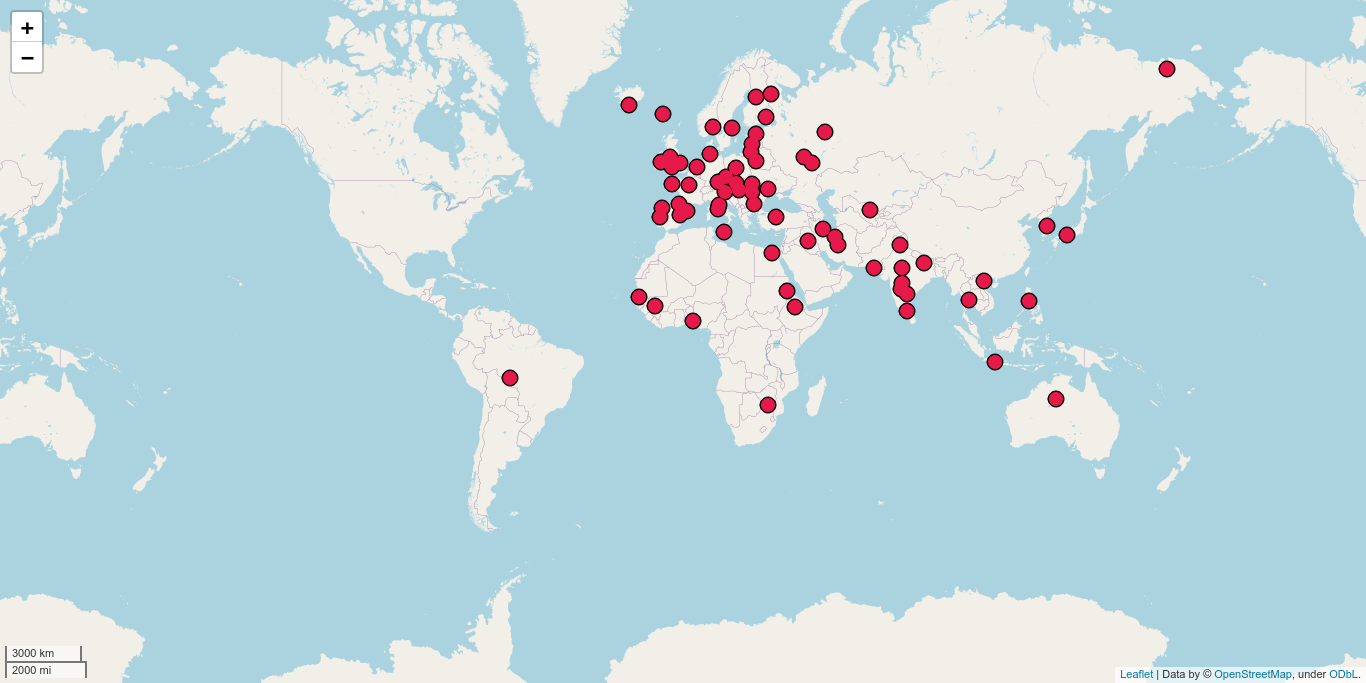
\includegraphics[scale=0.23]{images/map_ud2_8}
						\caption*{UD v2.8}
				\end{figure}
				\url{http://universaldependencies.org}
			}

			\only<2>{
 \begin{figure}
		\centering
		\begin{dependency}[theme=simple]
				\begin{deptext}[column sep = 0.8em]
						A \& cat \& chases \& rats \& and \& mice\\
				\end{deptext}
				\depedge{2}{1}{det}
				\depedge{3}{2}{nsubj}
				\depedge{3}{4}{dobj}
				\depedge{4}{5}{cc}
				\depedge{4}{6}{conj}
		\end{dependency}

				\quad

		\begin{dependency}[theme=simple]
				\begin{deptext}[column sep = 0.8em]
						En \& katt \& jagar \& råttor \& och \& möss\\
				\end{deptext}
				\depedge{2}{1}{DT}
				\depedge{3}{2}{SS}
				\depedge{5}{4}{CJ}
				\depedge{3}{5}{OO}
				\depedge{5}{6}{CJ}
		\end{dependency}

				\quad 

		\begin{dependency}[theme=simple]
				\begin{deptext}[column sep = 0.8em]
						En \& kat \& jager \& rotter \& og \& mus\\
				\end{deptext}
				\depedge{3}{1}{subj}
				\depedge{1}{2}{nobj}
				\depedge{3}{4}{dobj}
				\depedge{4}{5}{coord}
				\depedge{5}{6}{conj}
		\end{dependency}

				\caption*{Analyses syntaxiques originales pour la même phrase en anglais, suédois et danois.}
		\label{fig:diff_annot}
		% }

	\end{figure}
}
\only<3->{
	\begin{block}{}
		\begin{itemize}
	\item<3->let's annotate the same things the same way!
	\item<4->allow language-specific annotations
\end{itemize}
	\end{block}
}
\end{overlayarea}
\end{frame}

\begin{frame}{Comparaison}
\begin{table}[]
\begin{tabular}{l|l}
	\textbf{Dépendances}             & \textbf{Constituants}                 \\ 

	\hline
	\small{
		\begin{dependency}[theme=simple, edge style={gray}, label style={text=gray}]
			\begin{deptext}[column sep = 0.8em, nodes={text=gray}]
						I \& love \& syntax\\
				\end{deptext}
				\depedge{2}{1}{nsubj}
				\depedge{2}{3}{obj}
		\end{dependency}
	}
		&
		\tiny{
		\begin{forest}
			for tree={text=gray,edge=gray }
		[S 
			[NP 
				[ I ] 
			]
			[VP 
				[V 
					[love]
				]
				[NP 
					[syntax] 
				] 
			]
		]
	\end{forest}}\\
		\hline
Currently used more    & Historical importance        \\
Word order flexibility & More expressive              \\
Universal Dependencies & Many original datasets (e.g. PTB)

\end{tabular}
\end{table}
\end{frame}

\section{Pourquoi les analyseurs syntaxiques}

\begin{frame}{Question–Réponse}
\begin{overlayarea}{\textwidth}{0.6\textheight}
	\only<1>{
	\begin{figure}
		\centering
				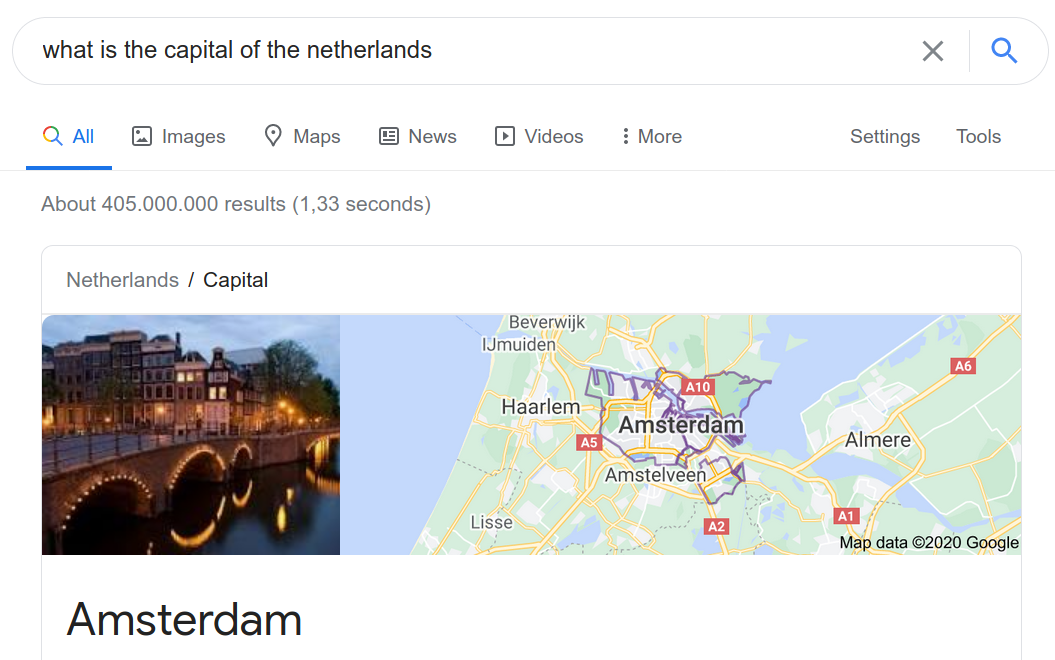
\includegraphics[scale=0.25]{images/qa1}
	\end{figure}
}
	\only<2>{
	\begin{figure}
		\centering
				
\includegraphics[scale=0.25]{images/qa3}
	\end{figure}
}
\end{overlayarea}
	
\end{frame}

\begin{frame}{Comprendre la question}
		\begin{overlayarea}{\textwidth}{0.6\textheight}

			\only<1>{
				\begin{figure}
						\begin{dependency}[theme=simple]
								\begin{deptext}[column sep=0.5em]
										Who \& developed \& the \& algorithm \& for \& the \& black \& hole \& image \\
										 \& \& \& \& \& \& \& \& \\
								\end{deptext}
								\depedge{2}{1}{nsubj}
								\deproot{2}{root}
								\depedge{4}{3}{det}
								\depedge{2}{4}{obj}
								\depedge{9}{5}{case}
								\depedge{9}{6}{det}
								\depedge{8}{7}{compound} %?
								\depedge{9}{8}{compound}
								\depedge{4}{9}{obl}
						\end{dependency}
				\end{figure}
			}

			\only<2>{
				\begin{figure}
						\begin{dependency}[theme=simple]
								\begin{deptext}[column sep=0.5em]
										Who \& developed \& the \& algorithm \& for \& the \& black \& hole \& image \\
										 \& \& \& \& \& \& \& \& \\
								\end{deptext}
								\depedge[red]{2}{1}{SUBJECT}
								\deproot{2}{root}
								\depedge{4}{3}{det}
								\depedge{2}{4}{obj}
								\depedge{9}{5}{case}
								\depedge{9}{6}{det}
								\depedge{8}{7}{compound} %?
								\depedge{9}{8}{compound}
								\depedge{4}{9}{obl}
						\end{dependency}
				\end{figure}
			}

			\only<3>{
				\begin{figure}
						\begin{dependency}[theme=simple]
								\begin{deptext}[column sep=0.5em]
										Who \& developed \& the \& algorithm \& for \& the \& black \& hole \& image \\
										 \& \& \& \& \& \& \& \& \\
								\end{deptext}
								\depedge{2}{1}{nsubj}
								\deproot{2}{root}
								\depedge{4}{3}{det}
								\depedge[red]{2}{4}{OBJECT}
								\depedge{9}{5}{case}
								\depedge{9}{6}{det}
								\depedge{8}{7}{compound} %?
								\depedge{9}{8}{compound}
								\depedge{4}{9}{obl}
						\end{dependency}
				\end{figure}
			}

			\only<4>{
				\begin{figure}
						\begin{dependency}[theme=simple]
								\begin{deptext}[column sep=0.5em]
										Who \& developed \& the \& algorithm \& for \& the \& black \& hole \& image \\
										 \& \& \& \& \& \& \& \& \\
								\end{deptext}
								\depedge{2}{1}{nsubj}
								\deproot{2}{root}
								\depedge{4}{3}{det}
								\depedge{2}{4}{obj}
								\depedge{9}{5}{case}
								\depedge{9}{6}{det}
								\depedge[red]{8}{7}{compound} %?
								\depedge{9}{8}{compound}
								\depedge{4}{9}{obl}
						\end{dependency}
				\end{figure}
			}

			\only<5>{
				\begin{figure}
						\begin{dependency}[theme=simple]
								\begin{deptext}[column sep=0.5em]
										Who \& developed \& the \& algorithm \& for \& the \& black \& hole \& image \\
										 \& \& \& \& \& \& \& \& \\
								\end{deptext}
								\depedge{2}{1}{nsubj}
								\deproot{2}{root}
								\depedge{4}{3}{det}
								\depedge{2}{4}{obj}
								\depedge{9}{5}{case}
								\depedge[red]{9}{6}{det}
								\depedge[red]{8}{7}{compound} %?
								\depedge[red]{9}{8}{compound}
								\depedge{4}{9}{obl}
						\end{dependency}
				\end{figure}
			}

			\only<6>{
				\begin{figure}
						\begin{dependency}[theme=simple]
								\begin{deptext}[column sep=0.5em]
										Who \& developed \& the \& algorithm \& for \& the \& black \& hole \& image \\
								\end{deptext}
								\depedge{2}{1}{nsubj}
								\deproot{2}{root}
								\depedge{4}{3}{det}
								\depedge{2}{4}{obj}
								\depedge[red]{9}{5}{case}
								\depedge[red]{9}{6}{det}
								\depedge[red]{8}{7}{compound} %?
								\depedge[red]{9}{8}{compound}
								\depedge[red]{4}{9}{obl}
						\end{dependency}
				\end{figure}
			}

			\only<7>{
				\begin{figure}
						\begin{dependency}[theme=simple]
								\begin{deptext}[column sep=0.5em]
										Who \& developed \& the \& algorithm \& for \& the \& black \& hole \& image \\
										 \& \& \& \& \& \& \& \& \\
								\end{deptext}
								\depedge{2}{1}{nsubj}
								\deproot{2}{root}
								\depedge{4}{3}{det}
								\depedge{2}{4}{obj}
								\depedge{9}{5}{case}
								\depedge{9}{6}{det}
								\depedge{8}{7}{compound} %?
								\depedge{9}{8}{compound}
								\depedge{4}{9}{obl}
						\end{dependency}
				\end{figure}
			}

			\only<8>{
				\begin{figure}
						\begin{dependency}[theme=simple]
								\begin{deptext}[column sep=0.5em]
										Who \& developed \& the \& algorithm \& for \& the \& black \& hole \& image \\
										 \& \& \& \& \& \& \& \& \\
								\end{deptext}
								\depedge{2}{1}{}
								\deproot{2}{}
								\depedge{4}{3}{}
								\depedge{2}{4}{}
								\depedge{9}{5}{}
								\depedge{9}{6}{}
								\depedge{8}{7}{} %?
								\depedge{9}{8}{}
								\depedge{4}{9}{}
						\end{dependency}
				\end{figure}
			}

			\end{overlayarea}
\end{frame}

\section{Analyseurs syntaxiques : comment}
\subsection{Algorithmes}

\begin{frame}{Parseurs à transitions}
\begin{overlayarea}{\textwidth}{0.6\textheight}
		\only<1>{
				\begin{figure}
						\centering
						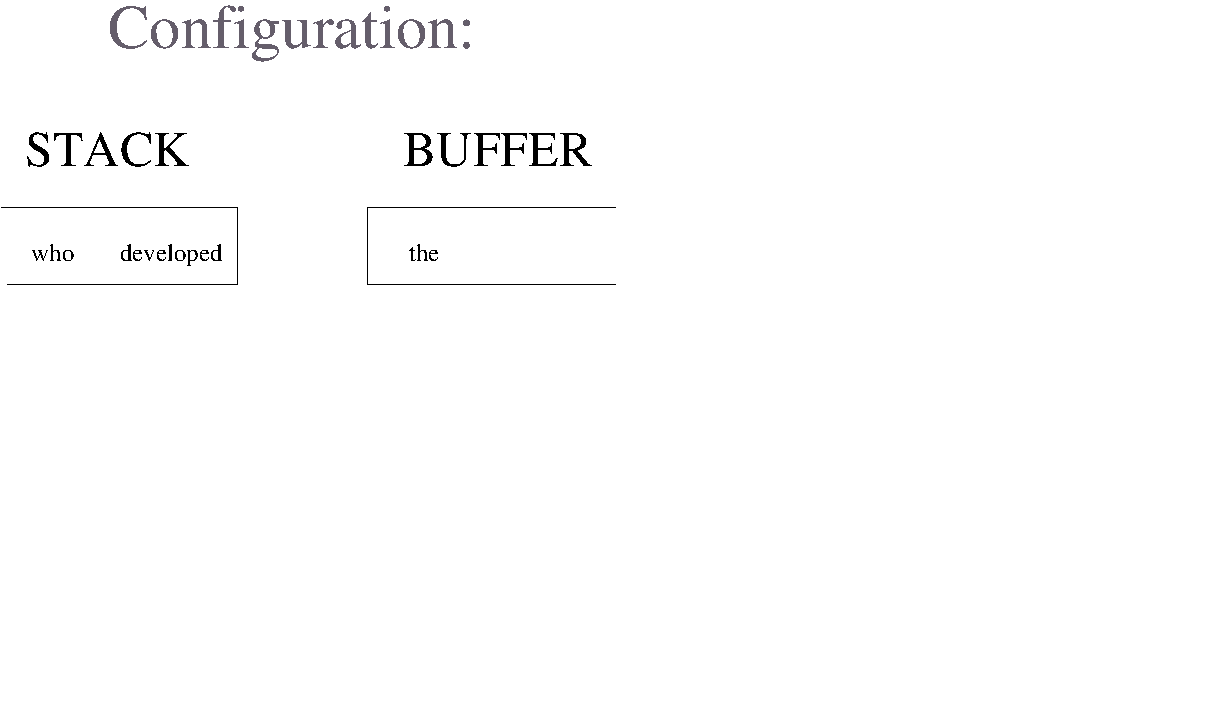
\includegraphics[scale=0.4]{images/trans2}
				\end{figure}
		}
		\only<2>{
				\begin{figure}
						\centering
						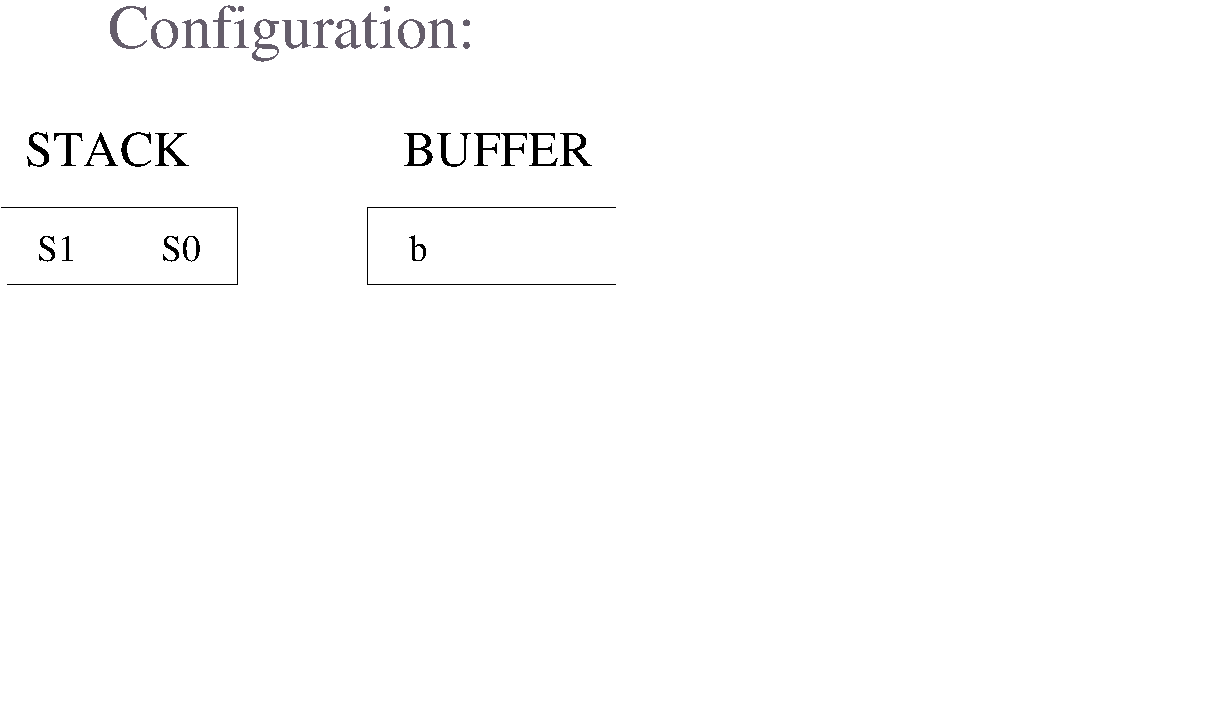
\includegraphics[scale=0.4]{images/trans3}
				\end{figure}
		}
		\only<3>{
				\begin{figure}
						\centering
						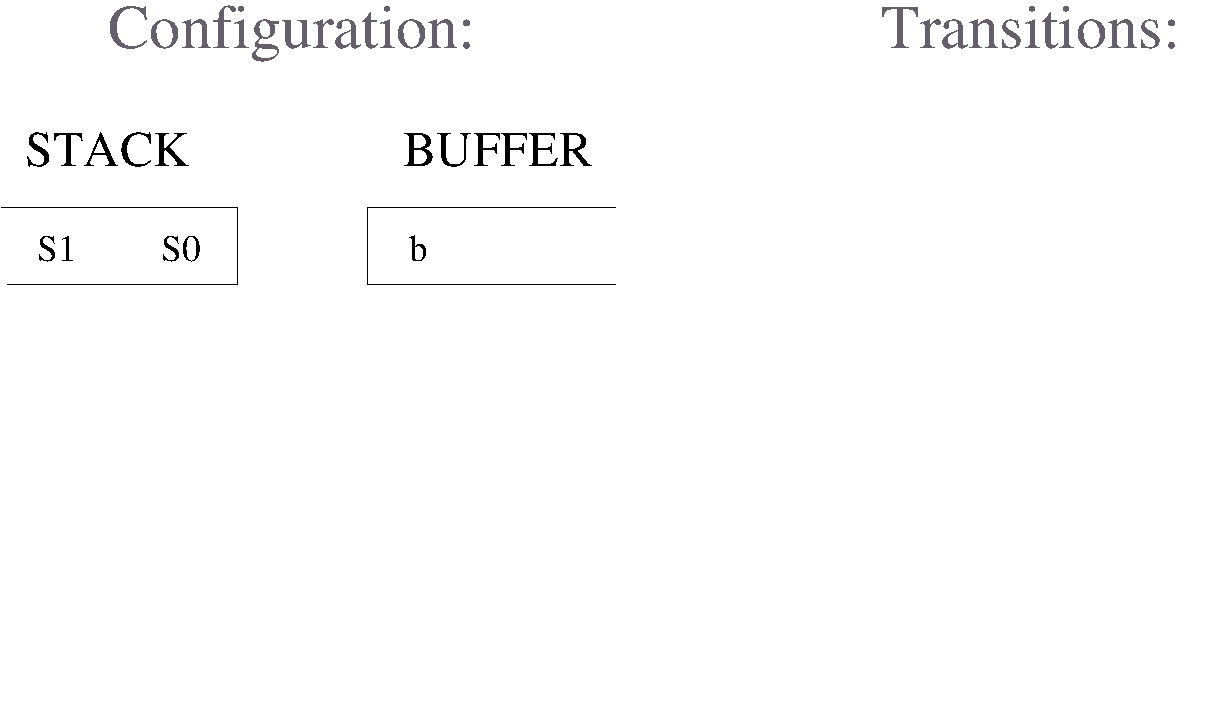
\includegraphics[scale=0.4]{images/trans4}
				\end{figure}
		}
		\only<4>{
				\begin{figure}
						\centering
						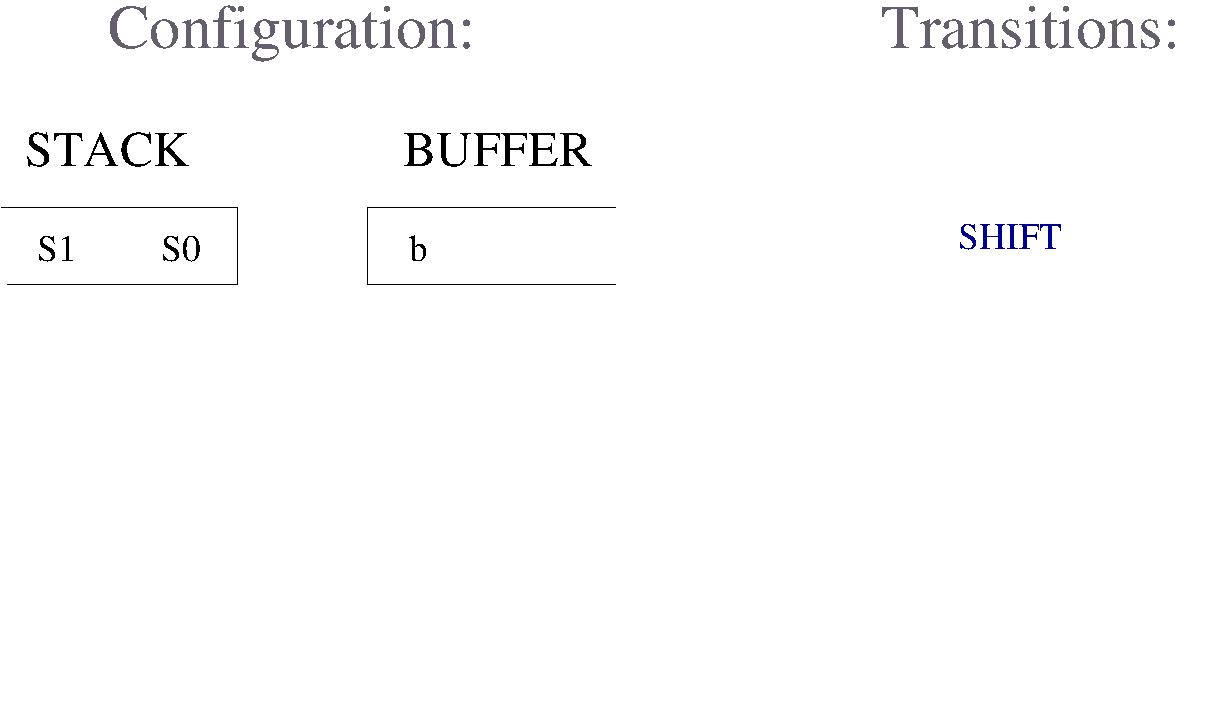
\includegraphics[scale=0.4]{images/trans5}
				\end{figure}
		}
		\only<5>{
				\begin{figure}
						\centering
						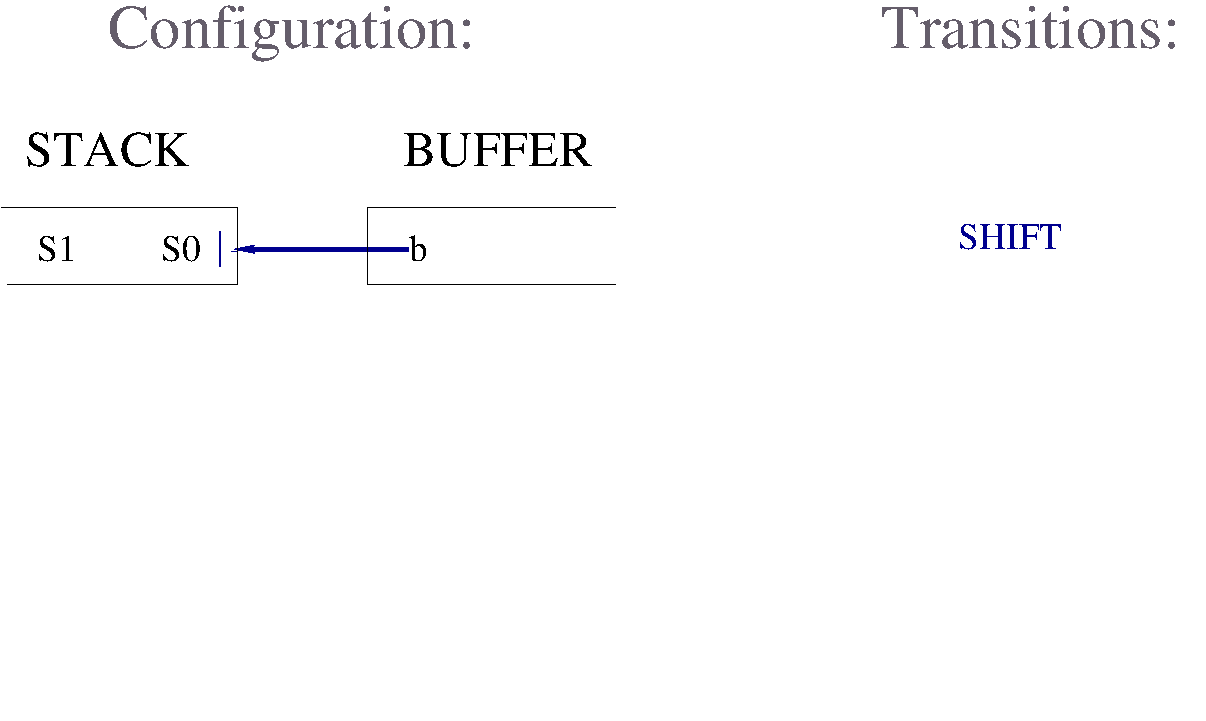
\includegraphics[scale=0.4]{images/trans6}
				\end{figure}
		}
		\only<6>{
				\begin{figure}
						\centering
						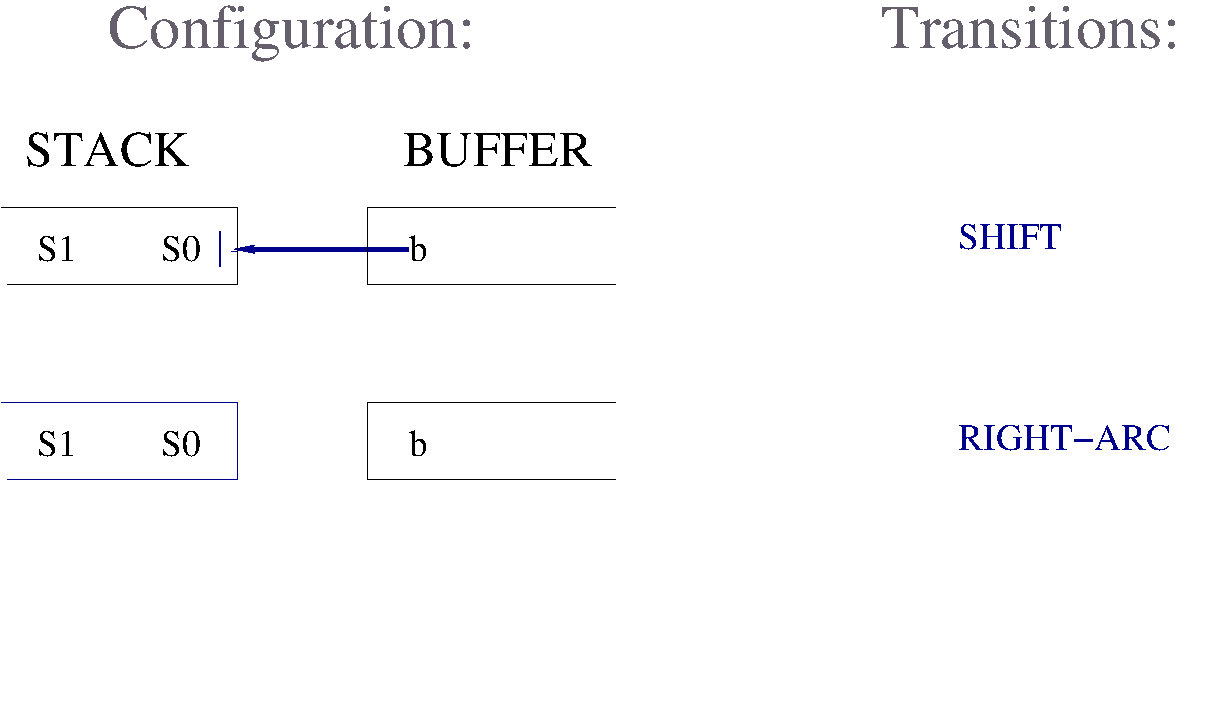
\includegraphics[scale=0.4]{images/trans7}
				\end{figure}
		}
		\only<7>{
				\begin{figure}
						\centering
						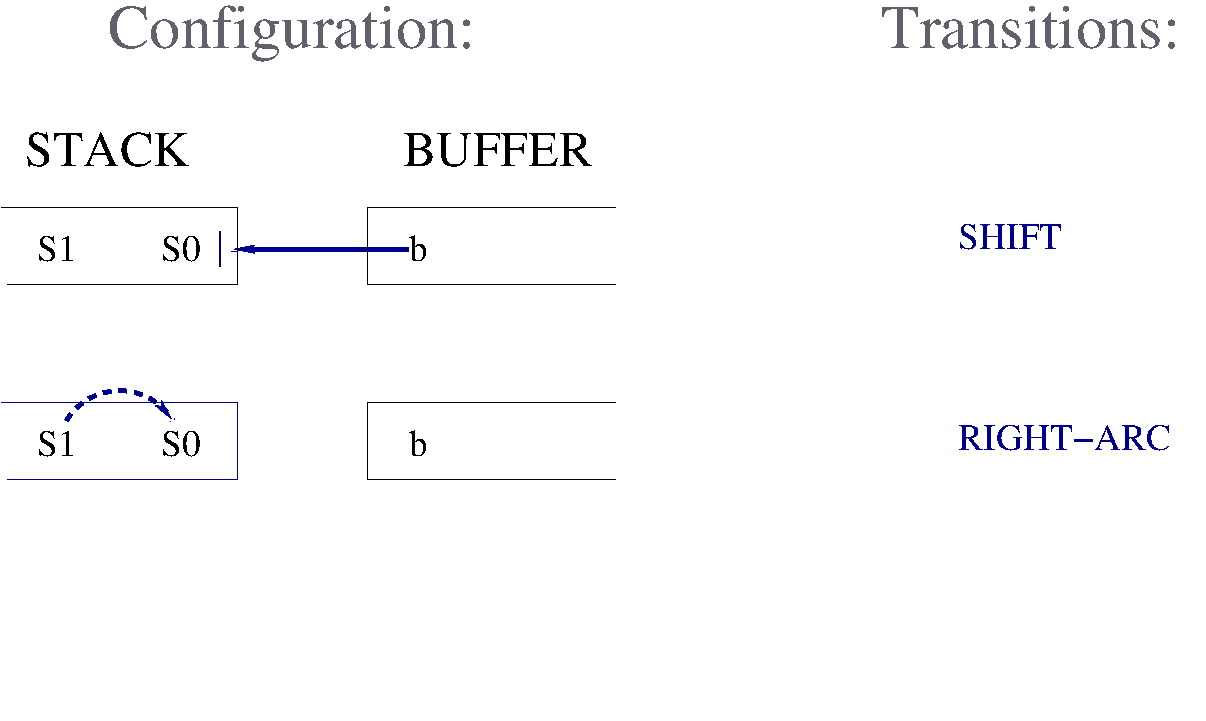
\includegraphics[scale=0.4]{images/trans8}
				\end{figure}
		}
		\only<8>{
				\begin{figure}
						\centering
						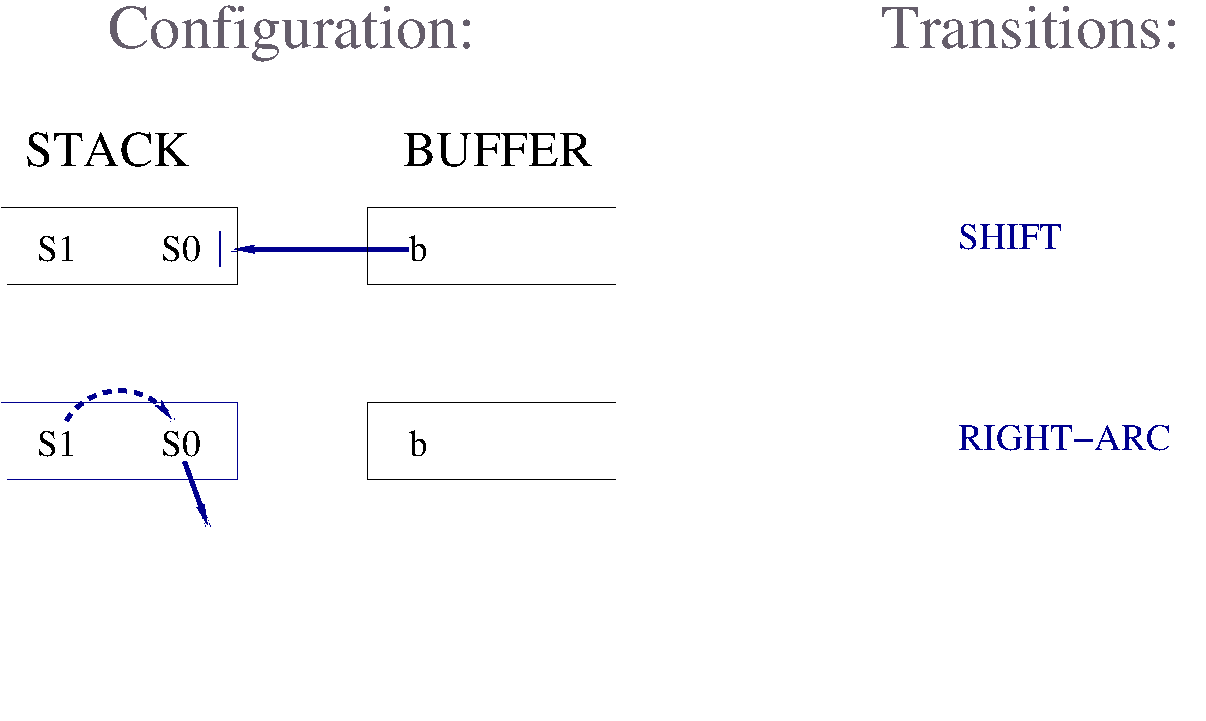
\includegraphics[scale=0.4]{images/trans9}
				\end{figure}
		}
		\only<9>{
				\begin{figure}
						\centering
						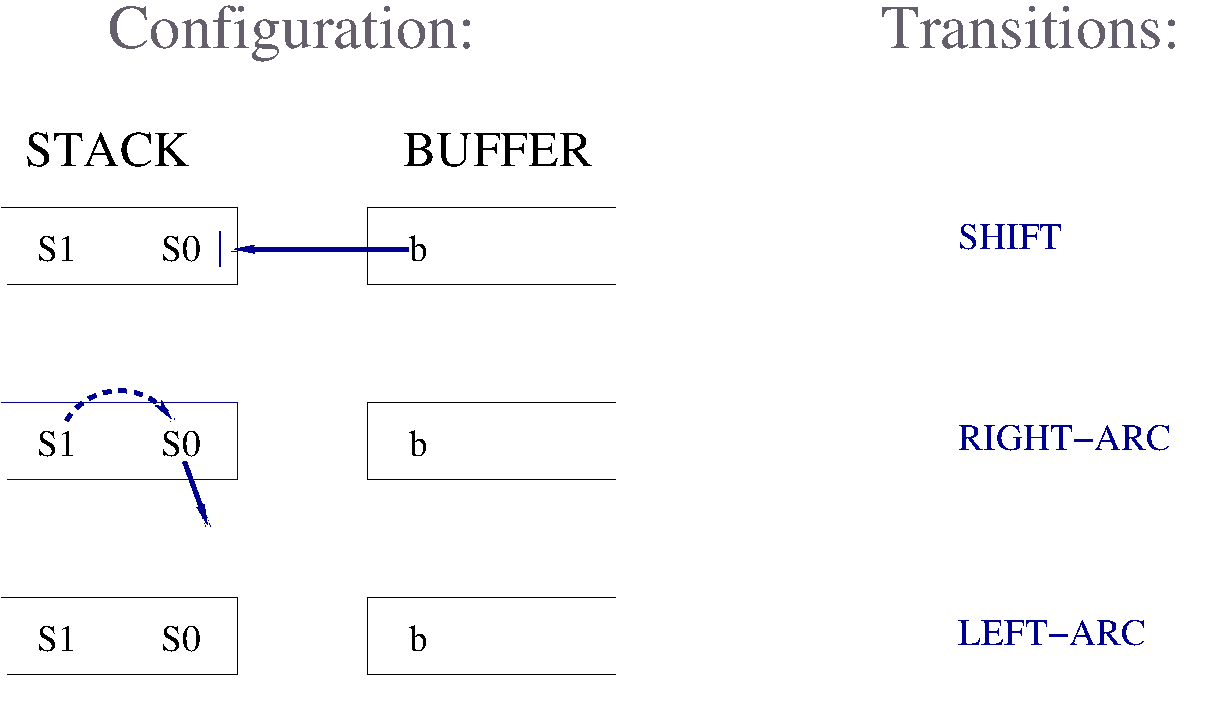
\includegraphics[scale=0.4]{images/trans10}
				\end{figure}
		}
		\only<10>{
				\begin{figure}
						\centering
						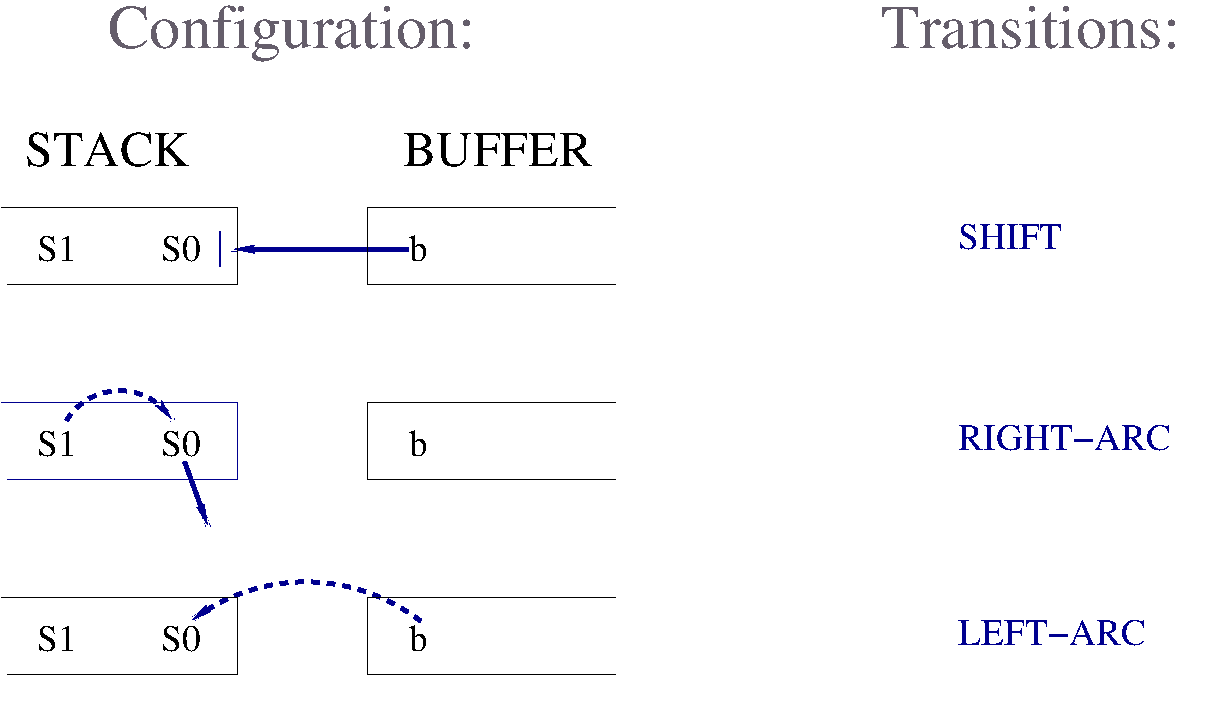
\includegraphics[scale=0.4]{images/trans11}
				\end{figure}
		}
		\only<11>{
				\begin{figure}
						\centering
						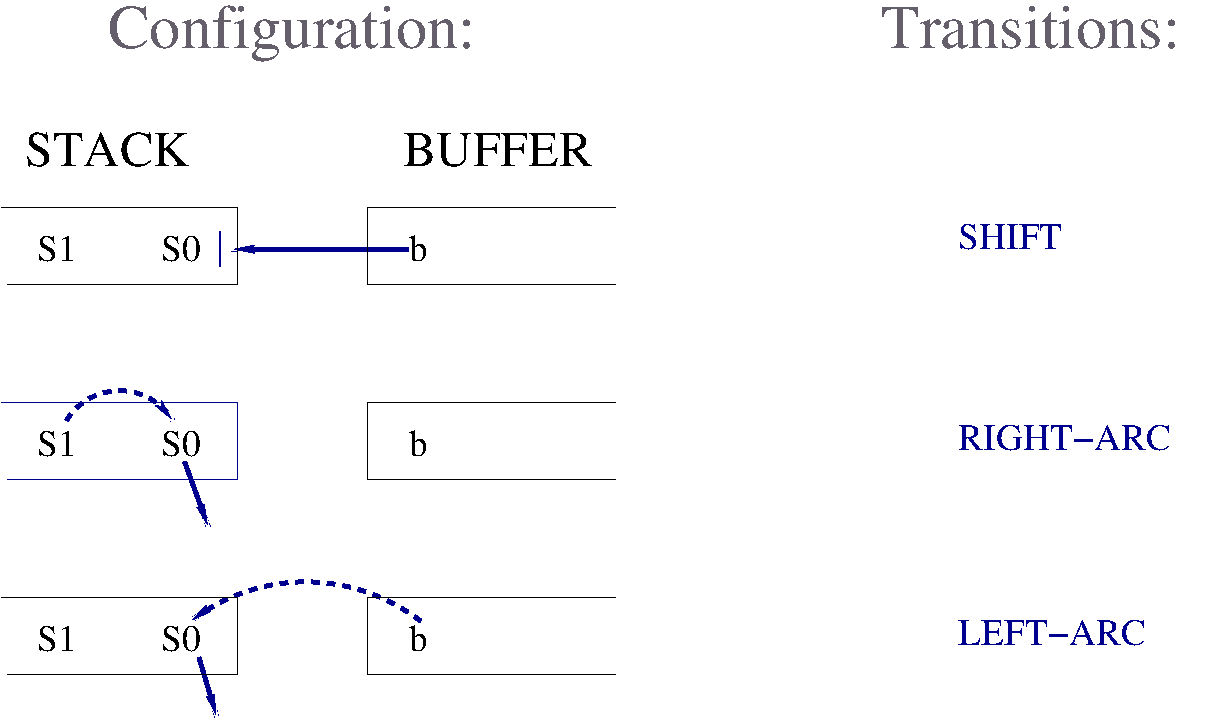
\includegraphics[scale=0.4]{images/trans12}
				\end{figure}
		}
		\vspace{1.5cm}
		\tiny{
		Arc-hybrid \parencite{kuhlmann-etal-2011-dynamic}
		}
	\end{overlayarea}
\end{frame}


\begin{frame}{Exemple}
\begin{overlayarea}{\textwidth}{0.8\textheight}
	\begin{columns}
		\begin{column}{0.65\textwidth}
				\only<1-3>{
						\begin{block}{}
								\vspace{0.27cm}
						\end{block}{}
				}
				\only<4>{
						\begin{block}{}
								\centerline{INITIAL CONFIGURATION}
						\end{block}{}
				}
				\only<5-6>{
						\begin{block}{}
								\centerline{\textcolor{lightgreen}{SHIFT}}
						\end{block}{}
				}
				\only<7>{
						\begin{block}{}
								\centerline{\textcolor{lightgreen}{LEFT-ARC}}
						\end{block}{}
				}
				\only<8>{
						\begin{block}{}
								\centerline{\textcolor{lightgreen}{SHIFT}}
						\end{block}{}
				}
				\only<9>{
						\begin{block}{}
								\centerline{\textcolor{lightgreen}{RIGHT-ARC}}
						\end{block}{}
				}
				\only<10>{
						\begin{block}{}
								\centerline{\textcolor{lightgreen}{SHIFT}}
						\end{block}{}
				}
				\only<11>{
						\begin{block}{}
								\centerline{\textcolor{lightgreen}{RIGHT-ARC}}
						\end{block}{}
				}
				\only<12>{
						\begin{block}{}
								\centerline{\textcolor{lightgreen}{LEFT-ARC}}
						\end{block}{}
				}
				\only<13>{
						\begin{block}{}
								\centerline{TERMINAL CONFIGURATION}
						\end{block}{}
					}

			\only<1>{
				\begin{figure}
						\begin{dependency}[theme=simple]
								\begin{deptext}[column sep=1em]
									Drive \& your \& friend \& home \& \textcolor{white}{**root**} \\
								\end{deptext}
								\depedge[white]{5}{1}{}
								\depedge[white]{3}{2}{}
								\depedge[white]{1}{3}{}
								\depedge[white]{1}{4}{}
								\deproot[white]{1}{}
						\end{dependency}
					\end{figure}
					}

			\only<2>{
				\begin{figure}
						\begin{dependency}[theme=simple]
								\begin{deptext}[column sep=1em]
									Drive \& your \& friend \& home \& \textcolor{white}{**root**} \\
								\end{deptext}
								\depedge[white]{5}{1}{}
								\depedge{3}{2}{}
								\depedge{1}{3}{}
								\depedge{1}{4}{}
								\deproot{1}{}
						\end{dependency}
					\end{figure}
					}

			\only<3>{
				\begin{figure}
						\begin{dependency}[theme=simple]
								\begin{deptext}[column sep=1em]
										Drive \& your \& friend \& home \& **root**\\
								\end{deptext}
								\depedge{5}{1}{}
								\depedge{3}{2}{}
								\depedge{1}{3}{}
								\depedge{1}{4}{}
						\end{dependency}
					\end{figure}
					}

				\only<4-6>{
				\begin{figure}
						\begin{dependency}[theme=simple]
								\begin{deptext}[column sep=1em]
										Drive \& your \& friend \& home \& **root**\\
								\end{deptext}
								\depedge{5}{1}{}
								\depedge{3}{2}{}
								\depedge{1}{3}{}
								\depedge{1}{4}{}
						\end{dependency}
				\end{figure}
				}

				\only<7-8>{
						\begin{figure}
								\begin{dependency}[theme=simple]
										\begin{deptext}[column sep=1em]
												Drive \& your \& friend \& home \& **root**\\
										\end{deptext}
										\depedge{5}{1}{}
										\depedge[green]{3}{2}{}
										\depedge{1}{3}{}
										\depedge{1}{4}{}
								\end{dependency}
						\end{figure}
				}

				\only<9-10>{
						\begin{figure}
								\begin{dependency}[theme=simple]
										\begin{deptext}[column sep=1em]
												Drive \& your \& friend \& home \& **root**\\
										\end{deptext}
										\depedge{5}{1}{}
										\depedge[green]{3}{2}{}
										\depedge[green]{1}{3}{}
										\depedge{1}{4}{}
								\end{dependency}
						\end{figure}
				}
				\only<11>{
						\begin{figure}
								\begin{dependency}[theme=simple]
										\begin{deptext}[column sep=1em]
												Drive \& your \& friend \& home \& **root**\\
										\end{deptext}
										\depedge{5}{1}{}
										\depedge[green]{3}{2}{}
										\depedge[green]{1}{3}{}
										\depedge[green]{1}{4}{}
								\end{dependency}
						\end{figure}
				}
				\only<12-13>{
						\begin{figure}
								\begin{dependency}[theme=simple]
										\begin{deptext}[column sep=1em]
												Drive \& your \& friend \& home \& **root**\\
										\end{deptext}
										\depedge[green]{5}{1}{}
										\depedge[green]{3}{2}{}
										\depedge[green]{1}{3}{}
										\depedge[green]{1}{4}{}
								\end{dependency}
						\end{figure}
				}

				\only<1-3>{
						\begin{block}{}
								\vspace{0.39cm}
						\end{block}
				}
				\only<4>{
				\begin{block}{}
						$[$ $]$ \hspace{0.9cm} $[$Drive your friend home **root**$]$
				\end{block}
				}
				\only<5>{
						\begin{block}{}
								$[$ Drive $]$ \hspace{0.9cm} $[$your friend home **root**$]$
						\end{block}
				}
				\only<6>{
						\begin{block}{}
								$[$ Drive your $]$ \hspace{0.9cm} $[$friend home **root**$]$
						\end{block}
				}
				\only<7>{
						\begin{block}{}
								$[$ Drive $]$ \hspace{0.9cm} $[$friend home **root**$]$\\
						\end{block}
				}
				\only<8>{
						\begin{block}{}
								$[$ Drive friend$]$ \hspace{0.9cm} $[$home **root**$]$\\
						\end{block}
				}
				\only<9>{
						\begin{block}{}
								$[$ Drive $]$ \hspace{0.9cm} $[$home **root**$]$\\
						\end{block}
				}
				\only<10>{
						\begin{block}{}
								$[$ Drive home$]$ \hspace{0.9cm} $[$**root**$]$\\
						\end{block}
				}
				\only<11>{
						\begin{block}{}
								$[$ Drive $]$ \hspace{0.9cm} $[$**root**$]$\\
						\end{block}
				}
				\only<12-13>{
						\begin{block}{}
								$[$ $]$ \hspace{0.9cm} $[$**root**$]$\\
						\end{block}
				}

			\end{column}
		%\vspace{1.5cm}

		\begin{column}{0.3\textwidth}
				\begin{figure}
						\centering
						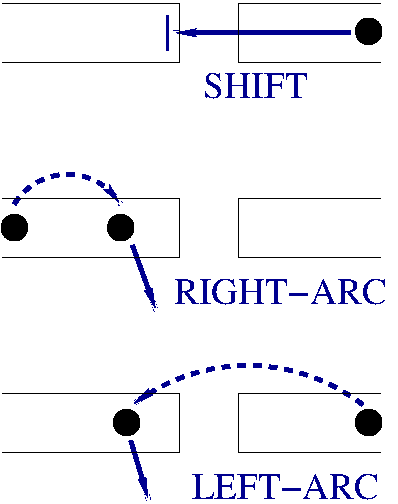
\includegraphics[scale=0.45]{images/transitions_b}
				\end{figure}
			\end{column}
		\end{columns}
\end{overlayarea}
\end{frame}

\begin{frame}{Entraîner un parseur à transitions}
		\only<1>{
				\begin{figure}
						\centering
						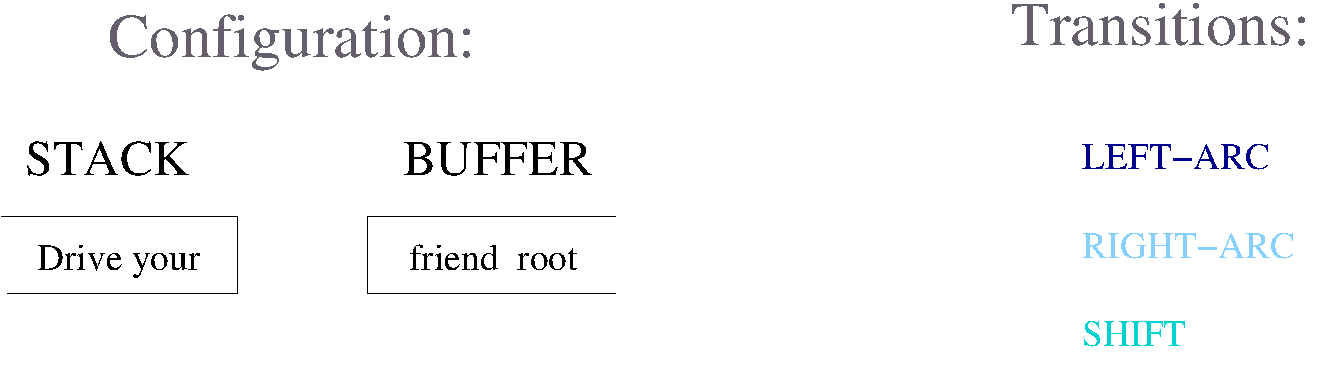
\includegraphics[scale=0.4]{images/trans_bonus_1}
				\end{figure}
		}
		\only<2>{
				\begin{figure}
						\centering
						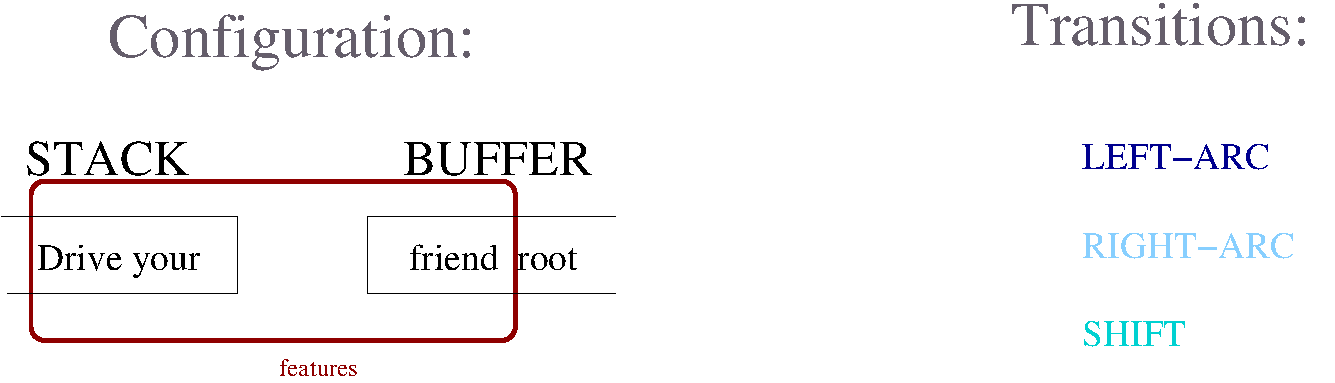
\includegraphics[scale=0.4]{images/trans_bonus_2}
				\end{figure}
		}
		\only<3>{
				\begin{figure}
						\centering
						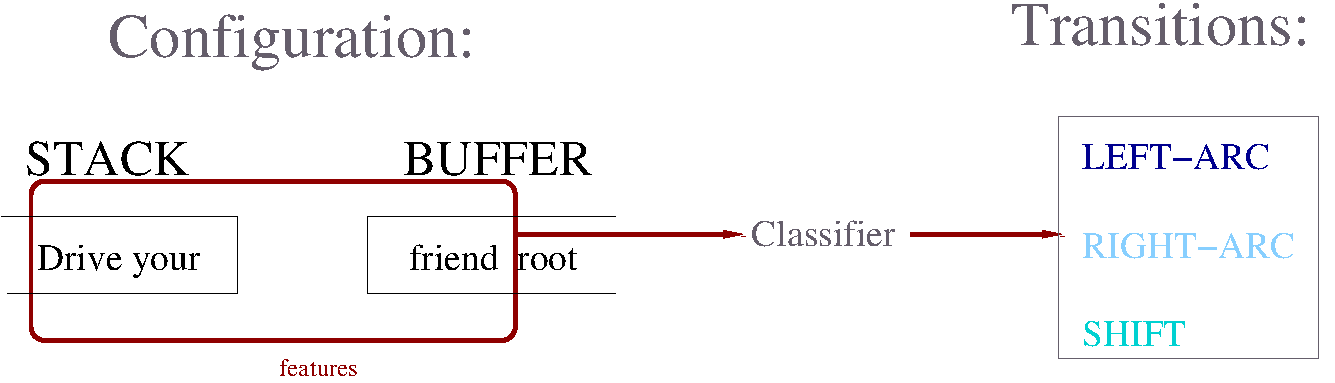
\includegraphics[scale=0.4]{images/trans_bonus_3}
				\end{figure}
		}
\end{frame}


\begin{frame}{À vous de jouer !}
	Trouver une séquence de transitions pour cet arbre
	\begin{figure}
		\begin{dependency}[theme=simple]
			\begin{deptext}[column sep=1em]
					I \& love \& parsing \& ! \& **root**\\
			\end{deptext}
			\depedge{2}{1}{}
			\depedge{5}{2}{}
			\depedge{2}{3}{}
			\depedge{2}{4}{}
		\end{dependency}
	\end{figure}
\end{frame}

\begin{frame}{Parseurs graphes}

\begin{overlayarea}{\textwidth}{0.8\textheight}
	\only<1-2>{
		\begin{block}{}
			\begin{itemize}
				\item<1-2> Score trees, not transitions
				\item<2> Factorize score into subtrees %add math?
			\end{itemize}
		\end{block}
	}

	\only<3>{
\begin{table}[]
\begin{tabular}{lrrrr}
	$d\downarrow$ $h\rightarrow$ & \multicolumn{1}{l}{\rotatebox{90}{root}}    & \multicolumn{1}{l}{\rotatebox{90}{I}}       & \multicolumn{1}{l}{\rotatebox{90}{love}}    & \multicolumn{1}{l}{\rotatebox{90}{syntax}}  \\
root   & \cellcolor[HTML]{C0C0C0}            & \cellcolor[HTML]{C0C0C0}   & \cellcolor[HTML]{C0C0C0}            & \cellcolor[HTML]{C0C0C0}   \\
I      & \cellcolor[HTML]{C9DAF8}0.1          & \cellcolor[HTML]{C0C0C0}   & \cellcolor[HTML]{6095EB}0.7 & \cellcolor[HTML]{BAD0F6}0.2 \\
love   & \cellcolor[HTML]{4A86E8}0.8 & \cellcolor[HTML]{C9DAF8}0.1 & \cellcolor[HTML]{C0C0C0}            & \cellcolor[HTML]{C9DAF8}0.1 \\
syntax & \cellcolor[HTML]{C9DAF8}0.1          & \cellcolor[HTML]{AAC6F5}0.3 & \cellcolor[HTML]{75A3EE}0.6 & \cellcolor[HTML]{C0C0C0}  
\end{tabular}
\end{table}
}

	\only<4>{
\begin{table}[]
\begin{tabular}{lrrrr}
	$d\downarrow$ $h\rightarrow$ & \multicolumn{1}{l}{\rotatebox{90}{root}}    & \multicolumn{1}{l}{\rotatebox{90}{I}}       & \multicolumn{1}{l}{\rotatebox{90}{love}}    & \multicolumn{1}{l}{\rotatebox{90}{syntax}}  \\
root   & \cellcolor[HTML]{C0C0C0}            & \cellcolor[HTML]{C0C0C0}   & \cellcolor[HTML]{C0C0C0}            & \cellcolor[HTML]{C0C0C0}   \\
I      & \cellcolor[HTML]{C9DAF8}0.1          & \cellcolor[HTML]{C0C0C0}   & \cellcolor[HTML]{6095EB}\textbf{0.7} & \cellcolor[HTML]{BAD0F6}0.2 \\
love   & \cellcolor[HTML]{4A86E8}0.8 & \cellcolor[HTML]{C9DAF8}0.1 & \cellcolor[HTML]{C0C0C0}            & \cellcolor[HTML]{C9DAF8}0.1 \\
syntax & \cellcolor[HTML]{C9DAF8}0.1          & \cellcolor[HTML]{AAC6F5}0.3 & \cellcolor[HTML]{75A3EE}0.6 & \cellcolor[HTML]{C0C0C0}  
\end{tabular}
\end{table}
}


	\only<5>{
\begin{table}[]
\begin{tabular}{lrrrr}
	$d\downarrow$ $h\rightarrow$ & \multicolumn{1}{l}{\rotatebox{90}{root}}    & \multicolumn{1}{l}{\rotatebox{90}{I}}       & \multicolumn{1}{l}{\rotatebox{90}{love}}    & \multicolumn{1}{l}{\rotatebox{90}{syntax}}  \\
root   & \cellcolor[HTML]{C0C0C0}            & \cellcolor[HTML]{C0C0C0}   & \cellcolor[HTML]{C0C0C0}            & \cellcolor[HTML]{C0C0C0}   \\
I      & \cellcolor[HTML]{C9DAF8}0.1          & \cellcolor[HTML]{C0C0C0}   & \cellcolor[HTML]{6095EB}\textbf{0.7} & \cellcolor[HTML]{BAD0F6}0.2 \\
love   & \cellcolor[HTML]{4A86E8}\textbf{0.8} & \cellcolor[HTML]{C9DAF8}0.1 & \cellcolor[HTML]{C0C0C0}            & \cellcolor[HTML]{C9DAF8}0.1 \\
syntax & \cellcolor[HTML]{C9DAF8}0.1          & \cellcolor[HTML]{AAC6F5}0.3 & \cellcolor[HTML]{75A3EE}0.6 & \cellcolor[HTML]{C0C0C0}  
\end{tabular}
\end{table}
}

	\only<6>{
\begin{table}[]
\begin{tabular}{lrrrr}
	$d\downarrow$ $h\rightarrow$ & \multicolumn{1}{l}{\rotatebox{90}{root}}    & \multicolumn{1}{l}{\rotatebox{90}{I}}       & \multicolumn{1}{l}{\rotatebox{90}{love}}    & \multicolumn{1}{l}{\rotatebox{90}{syntax}}  \\
root   & \cellcolor[HTML]{C0C0C0}            & \cellcolor[HTML]{C0C0C0}   & \cellcolor[HTML]{C0C0C0}            & \cellcolor[HTML]{C0C0C0}   \\
I      & \cellcolor[HTML]{C9DAF8}0.1          & \cellcolor[HTML]{C0C0C0}   & \cellcolor[HTML]{6095EB}\textbf{0.7} & \cellcolor[HTML]{BAD0F6}0.2 \\
love   & \cellcolor[HTML]{4A86E8}\textbf{0.8} & \cellcolor[HTML]{C9DAF8}0.1 & \cellcolor[HTML]{C0C0C0}            & \cellcolor[HTML]{C9DAF8}0.1 \\
syntax & \cellcolor[HTML]{C9DAF8}0.1          & \cellcolor[HTML]{AAC6F5}0.3 & \cellcolor[HTML]{75A3EE}\textbf{0.6} & \cellcolor[HTML]{C0C0C0}  
\end{tabular}
\end{table}
}

\only<3>{
\begin{figure}
		\centering
		\begin{dependency}[theme=simple]
				\begin{deptext}[column sep = 0.8em]
						I \& love \& syntax\\
				\end{deptext}
				\depedge[white]{2}{1}{}
				\depedge[white]{2}{3}{}
				\deproot[white]{2}{}
		\end{dependency}
\end{figure}
}

\only<4>{
\begin{figure}
		\centering
		\begin{dependency}[theme=simple]
				\begin{deptext}[column sep = 0.8em]
						I \& love \& syntax\\
				\end{deptext}
				\depedge{2}{1}{}
				\depedge[white]{2}{3}{}
				\deproot[white]{2}{}
		\end{dependency}
\end{figure}
}

\only<5>{
\begin{figure}
		\centering
		\begin{dependency}[theme=simple]
				\begin{deptext}[column sep = 0.8em]
						I \& love \& syntax\\
				\end{deptext}
				\depedge{2}{1}{}
				\depedge[white]{2}{3}{}
				\deproot{2}{}
		\end{dependency}
\end{figure}
}

\only<6>{
\begin{figure}
		\centering
		\begin{dependency}[theme=simple]
				\begin{deptext}[column sep = 0.8em]
						I \& love \& syntax\\
				\end{deptext}
				\depedge{2}{1}{}
				\depedge{2}{3}{}
				\deproot{2}{}
		\end{dependency}
\end{figure}
}

\only<7->{
	\begin{block}{}
		\begin{itemize}
			\item<7-> Not as easy as picking the highest scoring head for each word
			\item<8-> Maximum Spanning Tree (MST) algorithm: find the highest scoring tree \parencite{mcdonald05tech}
			\item<9-> Using dynamic programming
		\end{itemize}
	\end{block}
}

\end{overlayarea}
\end{frame}

\subsection{Architectures}

\begin{frame}{Analyse syntaxique neuronale}
		\begin{overlayarea}{\textwidth}{\textheight}
	\only<1>{
	\begin{figure}
		\centering
		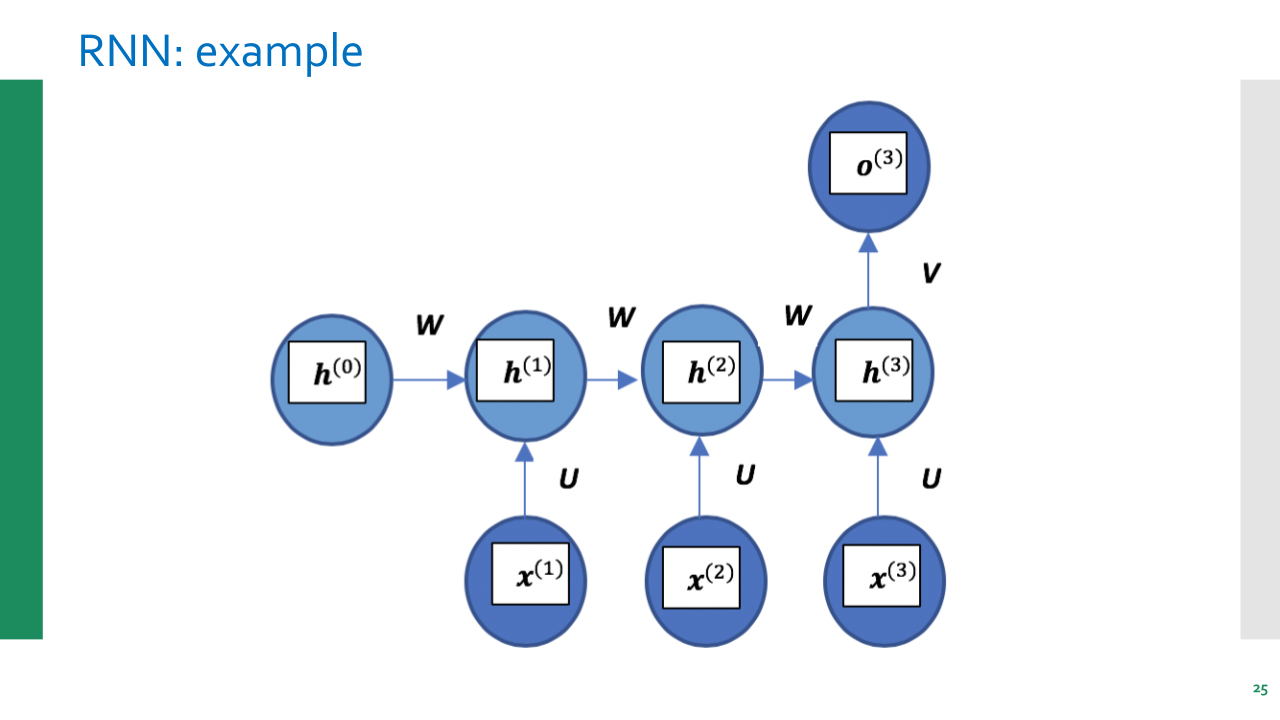
\includegraphics[scale=0.3]{images/rnn}
	\end{figure}
}
	\only<2>{
	\begin{figure}
		\centering
		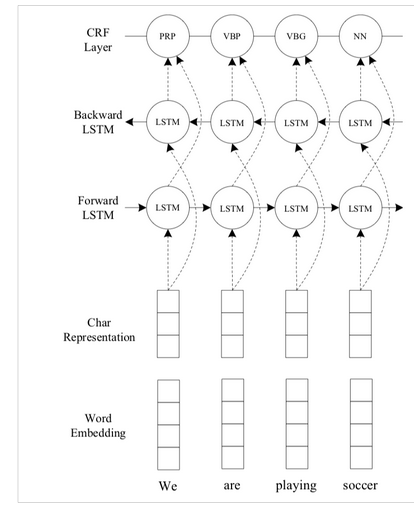
\includegraphics[scale=0.4]{images/lstm}
	\end{figure}
}
				\only<3>{
				\begin{figure}
						\centering
						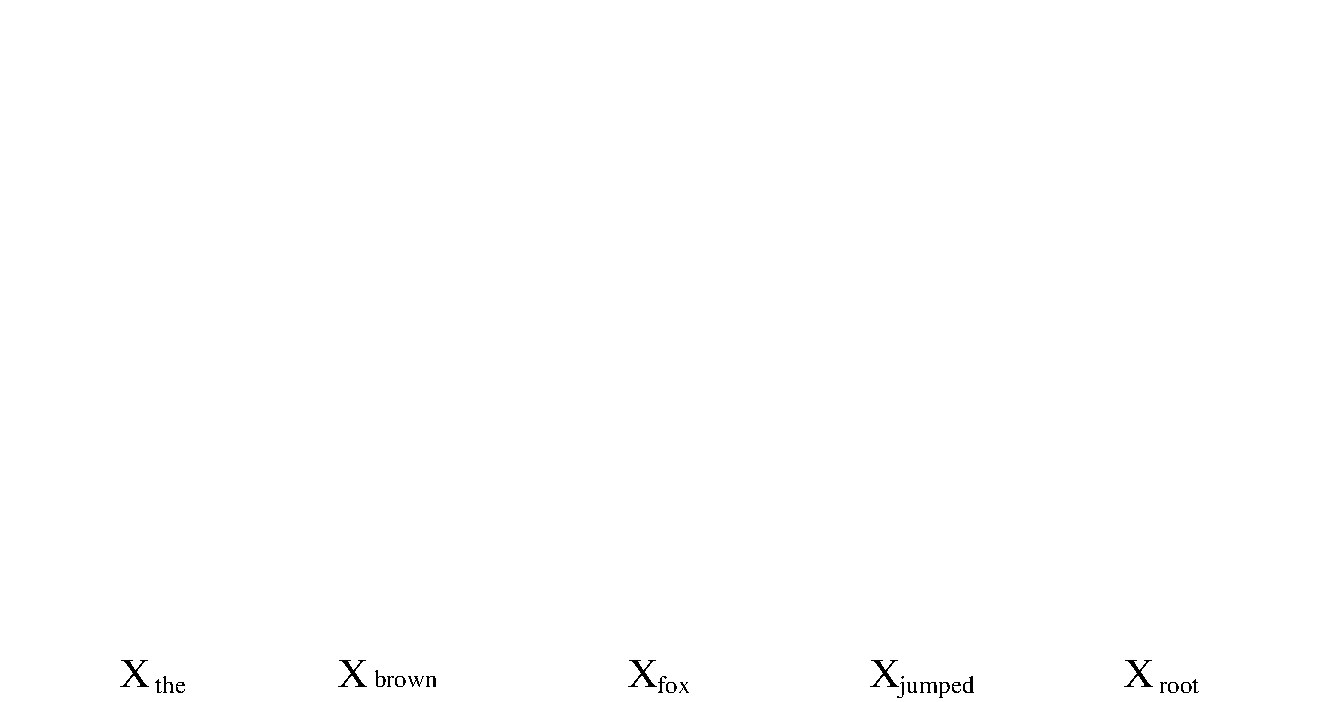
\includegraphics[scale=0.5]{images/1}
				\end{figure}
				}
				\only<4>{
				\begin{figure}
						\centering
						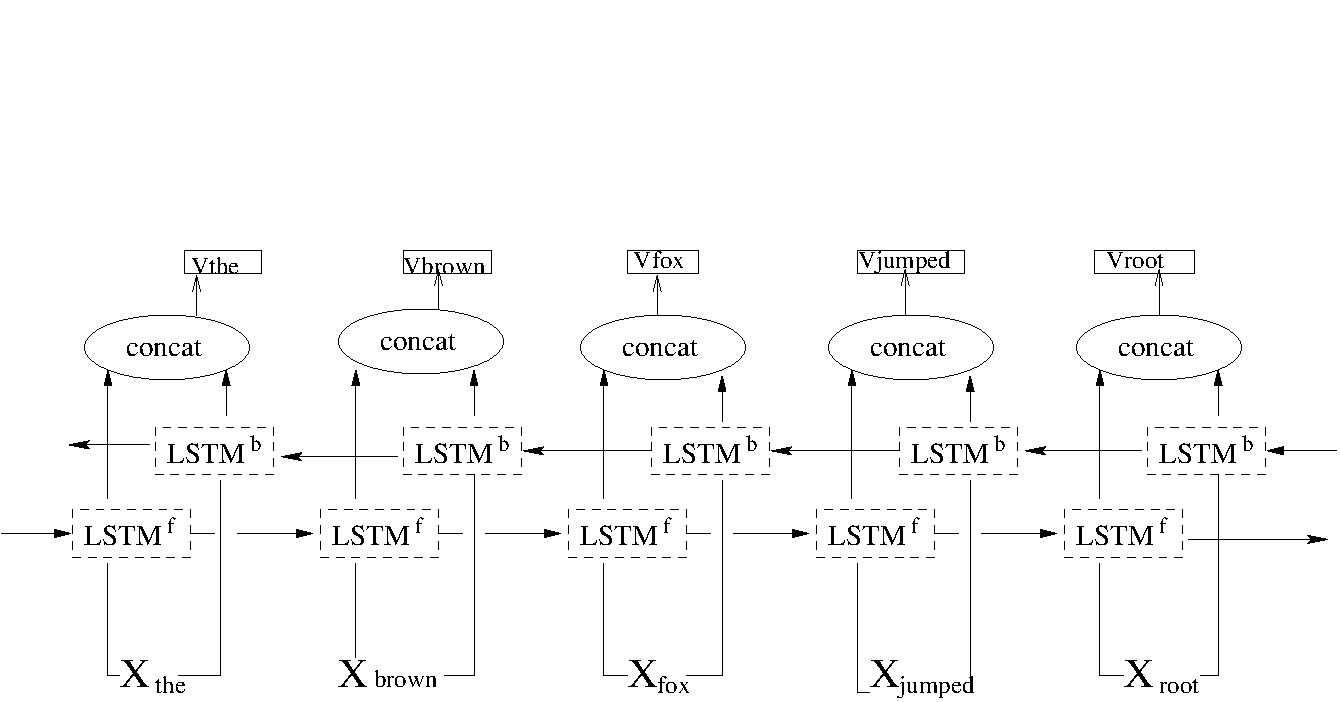
\includegraphics[scale=0.5]{images/2}
				\end{figure}
				}
				\only<5>{
				\begin{figure}
						\centering
						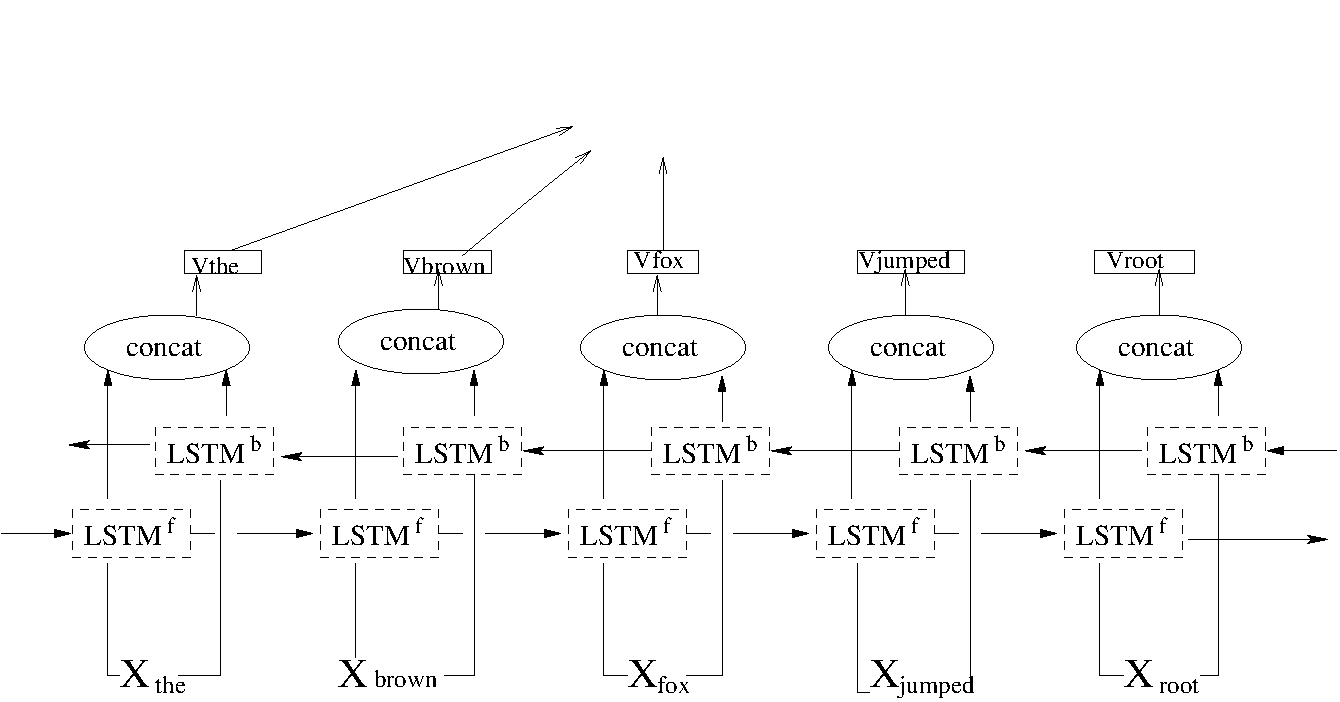
\includegraphics[scale=0.5]{images/3}
				\end{figure}
				}
				\only<6>{
				\begin{figure}
						\centering
						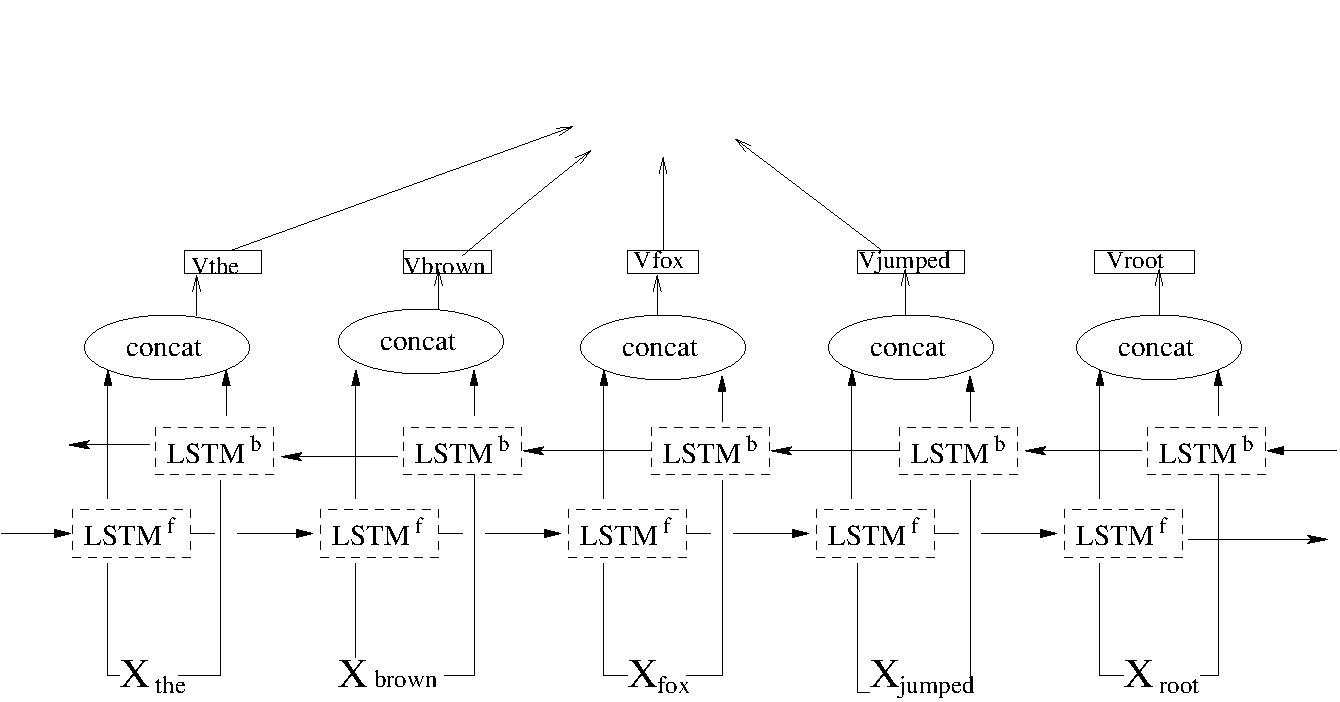
\includegraphics[scale=0.5]{images/4}
				\end{figure}
				}
				\only<7>{
				\begin{figure}
						\centering
						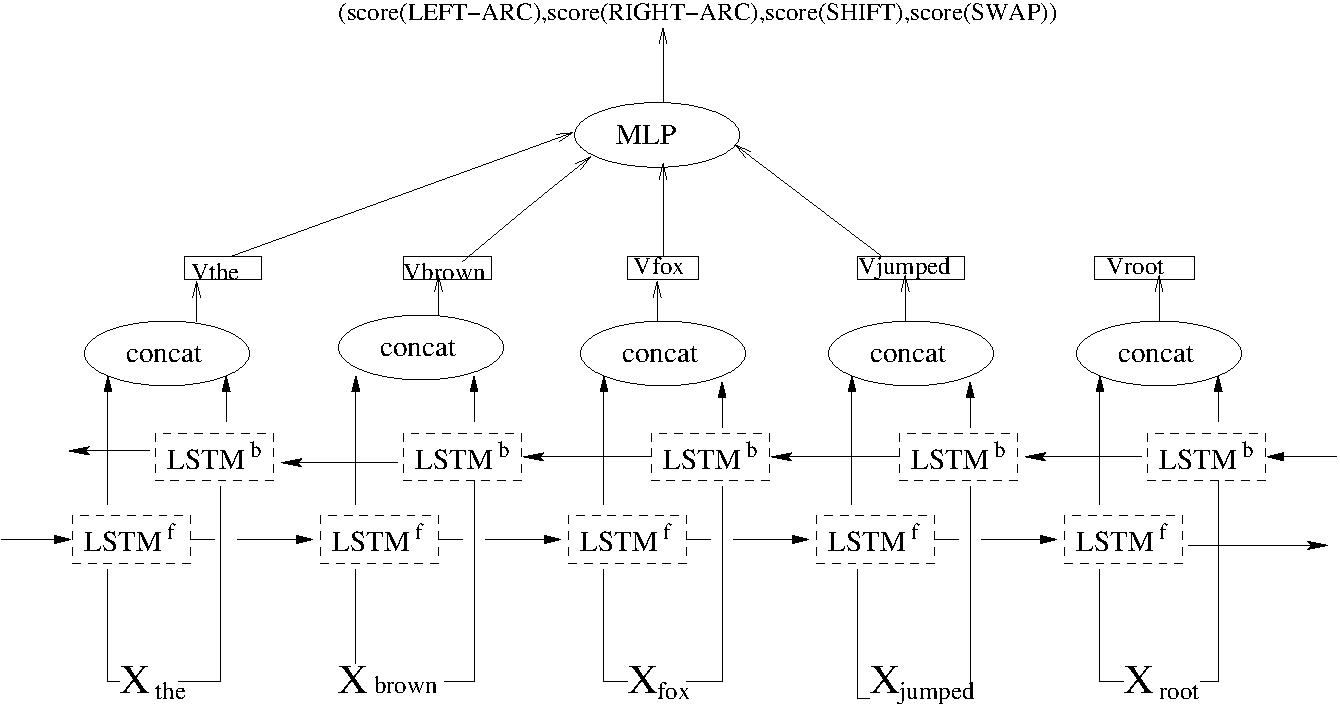
\includegraphics[scale=0.5]{images/5}
				\end{figure}
				}
				\only<8-9>
				{
\begin{table}[]
	\vspace{-0.5cm}
	\hspace{-1cm}
	\tiny
	\centering
\begin{tabular}{lrrrrr}
	& \multicolumn{1}{l}{\rotatebox{45}{root}}    & \multicolumn{1}{l}{\rotatebox{45}{the}}     & \multicolumn{1}{l}{\rotatebox{45}{brown}}   & \multicolumn{1}{l}{\rotatebox{45}{fox}}     & \multicolumn{1}{l}{\rotatebox{45}{jumped}}  \\
root   & \cellcolor[HTML]{C0C0C0}{\color[HTML]{C0C0C0} } & \cellcolor[HTML]{C0C0C0}                        & \cellcolor[HTML]{C0C0C0}                        & \cellcolor[HTML]{C0C0C0}                        & \cellcolor[HTML]{C0C0C0}                        \\
the    & \cellcolor[HTML]{C9DAF8}0.1                     & \cellcolor[HTML]{C0C0C0}{\color[HTML]{C0C0C0} } & \cellcolor[HTML]{C9DAF8}0.1                     & \cellcolor[HTML]{6095EB}0.7                     & \cellcolor[HTML]{C9DAF8}0.1                     \\
brown  & \cellcolor[HTML]{C9DAF8}0.1                     & \cellcolor[HTML]{C9DAF8}0.1                     & \cellcolor[HTML]{C0C0C0}{\color[HTML]{C0C0C0} } & \cellcolor[HTML]{75A3EE}0.6                     & \cellcolor[HTML]{C9DAF8}0.1                     \\
fox    & \cellcolor[HTML]{C9DAF8}0.1                     & \cellcolor[HTML]{AAC6F5}0.3                     & \cellcolor[HTML]{C9DAF8}0.1                     & \cellcolor[HTML]{C0C0C0}{\color[HTML]{C0C0C0} } & \cellcolor[HTML]{8AB0F0}0.5                     \\
jumped & \cellcolor[HTML]{6095EB}0.7                     & \cellcolor[HTML]{C9DAF8}0.1                     & \cellcolor[HTML]{C9DAF8}0.1                     & \cellcolor[HTML]{C9DAF8}0.1                     & \cellcolor[HTML]{C0C0C0}{\color[HTML]{C0C0C0} }
\end{tabular}
\end{table}
\vspace{-0.5cm}
}
\only<8>{
				\begin{figure}
						\centering
						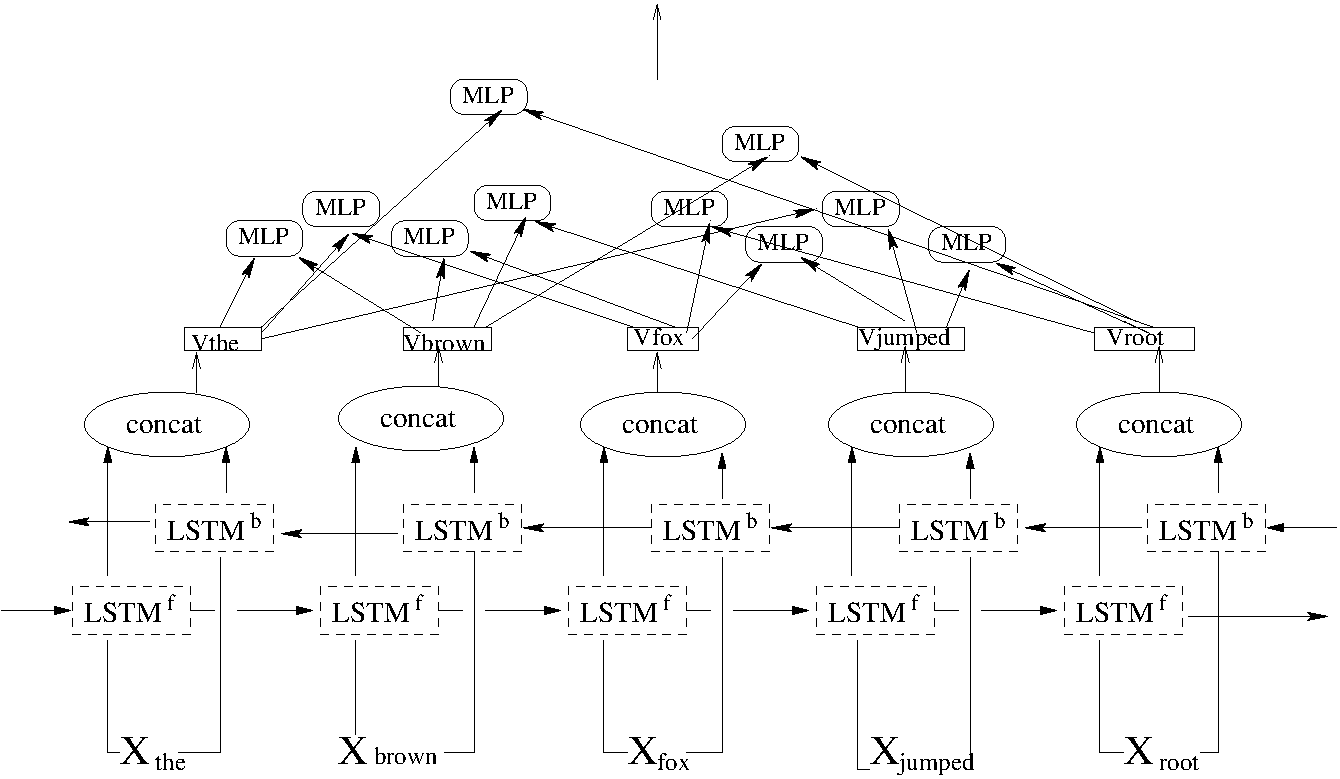
\includegraphics[scale=0.4]{images/archit_gb}
				\end{figure}
			}

		\only<2-7>{
		\vspace{1cm}
		}
		\only<3-8>{
		\tiny{
		\textcite{kiperwasser16}
		}
	}
\end{overlayarea}
\end{frame}

\begin{frame}{Transition vs. Graphe}
		\begin{overlayarea}{\textwidth}{0.6\textheight}
	\begin{columns}
		\begin{column}{0.45\textwidth}
			\begin{block}{Transition-based}
				\begin{itemize}
					\item<2-> Greedy search
					\item<3-> Faster
				\end{itemize}
			\end{block}
		\end{column}
		\begin{column}{0.45\textwidth}
			\begin{block}{Graph-based}
				\begin{itemize}
					\item<2-> Exact search
					\item<3-> More accurate
				\end{itemize}
			\end{block}
		\end{column}
	\end{columns}
	\only<4>{
	\begin{block}{}
		In the neural era, the differences between the two paradigms decreased \parencite{kulmizev19deep}.
		%TODO: could also cite Hewitt & Manning but would maybe be too much
	\end{block}
	}
\end{overlayarea}
\end{frame}

\begin{frame}{Réseaux récurrents}
		\only<1>{
				\begin{figure}
						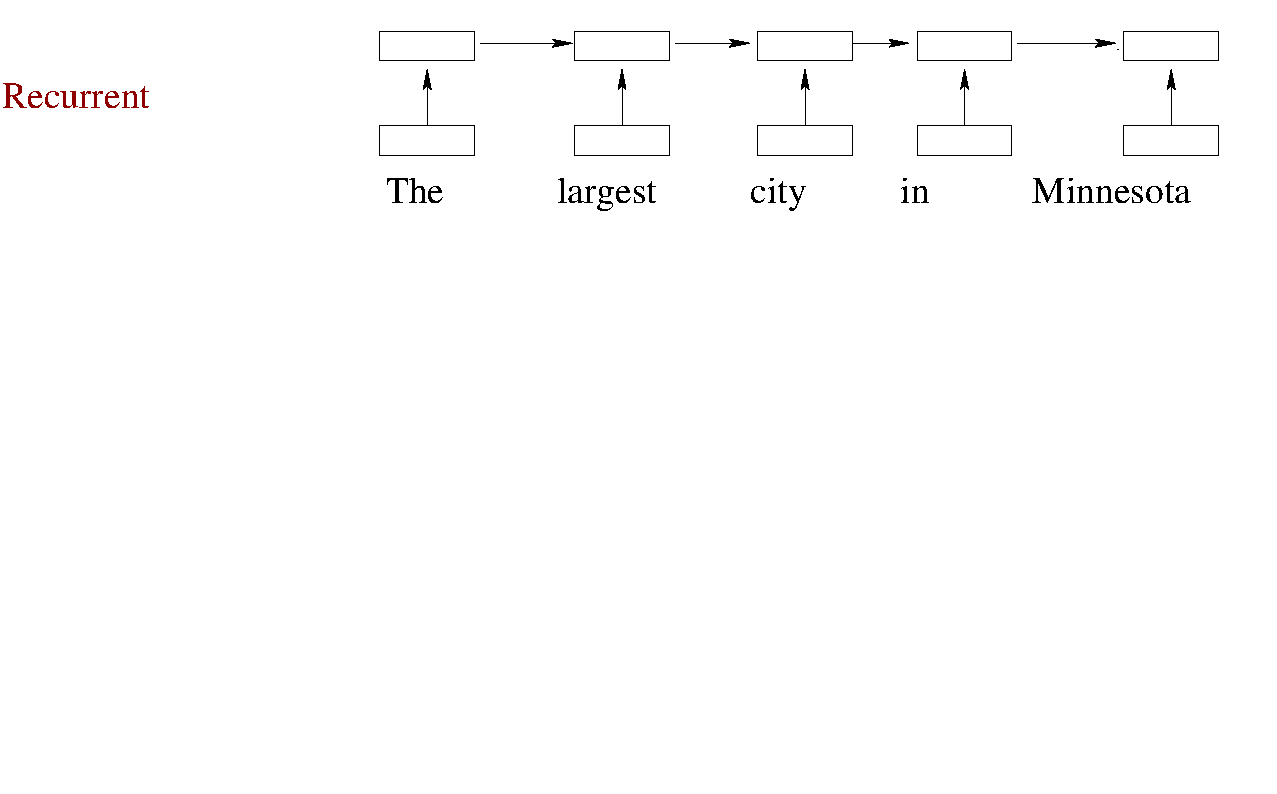
\includegraphics[scale=0.4]{images/recursive_vs_recurrent_1}
				\end{figure}
		}
		\only<2>{
				\begin{figure}
						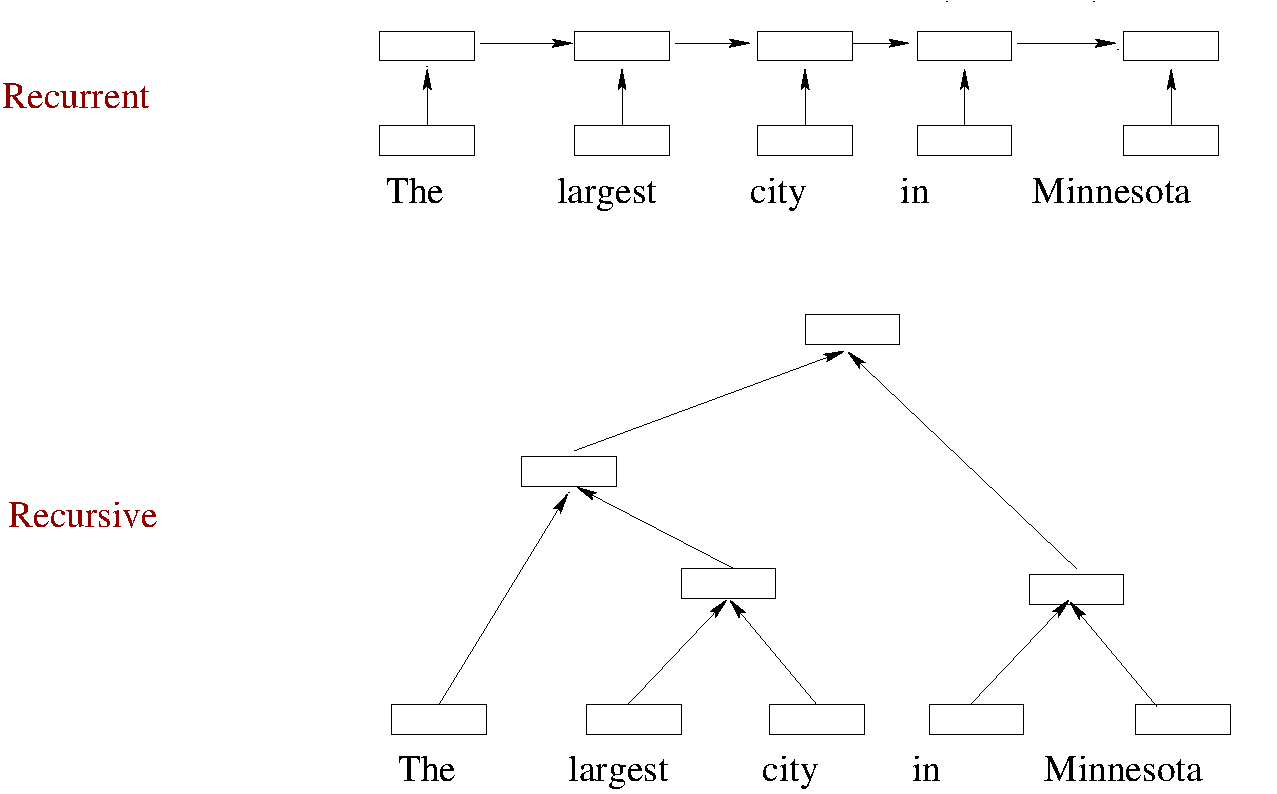
\includegraphics[scale=0.4]{images/recursive_vs_recurrent_2}
				\end{figure}
		}

\end{frame}

\begin{frame}{Réseaux récurrents pour analyseurs à transitions}
		\begin{overlayarea}{\textwidth}{0.6\textheight}

				\only<1>{
						\begin{figure}
								\begin{dependency}[theme=simple]
										\begin{deptext}[column sep=1em]
												the \& largest \& city\\
												\textcolor{white}{left-arc}\& \textcolor{white}{left-arc}\& \\
										\end{deptext}
										\depedge[white]{3}{2}{}
										\depedge[white]{3}{1}{}
								\end{dependency}
						\end{figure}
				}

				\only<2>{
				\begin{figure}
						\begin{dependency}[theme=simple]
								\begin{deptext}[column sep=1em]
										the \& largest \& city\\
										\textcolor{white}{left-arc}\& \textcolor{bordeaux}{left-arc}\& \\
								\end{deptext}
								\depedge{3}{2}{nmod}
								\depedge[white]{3}{1}{}
						\end{dependency}
				\end{figure}
				}

				\only<3>{
						\begin{figure}
								\begin{dependency}[theme=simple]
										\begin{deptext}[column sep=1em]
												the \& largest \& city\\
												\textcolor{bordeaux}{left-arc}\& \textcolor{white}{left-arc}\& \\
										\end{deptext}
										\depedge{3}{2}{nmod}
										\depedge{3}{1}{det}
								\end{dependency}
						\end{figure}
				}

				\only<4-6>{
						\begin{figure}
								\begin{dependency}[theme=simple]
										\begin{deptext}[column sep=1em]
												the \& largest \& city\\
												\textcolor{white}{left-arc}\& \textcolor{white}{left-arc}\& \\
										\end{deptext}
										\depedge{3}{2}{nmod}
										\depedge{3}{1}{det}
								\end{dependency}
						\end{figure}
				}

				\only<7>{
						\begin{figure}
								\begin{dependency}[theme=simple]
										\begin{deptext}[column sep=1em]
												the \& largest \& city\\
												\textcolor{white}{left-arc}\& \textcolor{white}{left-arc}\& \\
										\end{deptext}
										\depedge[red]{3}{2}{nmod}
										\depedge{3}{1}{det}
								\end{dependency}
						\end{figure}
				}

				\only<8>{
						\begin{figure}
								\begin{dependency}[theme=simple]
										\begin{deptext}[column sep=1em]
												the \& largest \& city\\
												\textcolor{white}{left-arc}\& \textcolor{white}{left-arc}\& \\
										\end{deptext}
										\depedge{3}{2}{nmod}
										\depedge[red]{3}{1}{det}
								\end{dependency}
						\end{figure}
				}

		\only<4->{
				\footnotesize{
						Recursive composition function \parencite{dyer15}:}\\
		}
		\begin{flalign*}
				\centering
				\only<5->{c(h,d,r) &= tanh(W[h;d;r]+b) \textcolor{white}{W[city, largest, left-nmod]}\\} 
				\only<6>{h_i &= c(h_{i-1},d,r) \textcolor{white}{W[city, largest, left-nmod]}\\} 
				\only<7->{city_1 &= c(city_0, largest, left-nmod)\\}
				\only<8->{city_2 &=c(city_1, the, left-det) }
		\end{flalign*}
		%}
\end{overlayarea}
\end{frame}
%TODO: add stack lstm and our results?

\begin{frame}{Composition récursive dans un BiLSTM}

		\only<1>{
				\begin{figure}
						\centering
						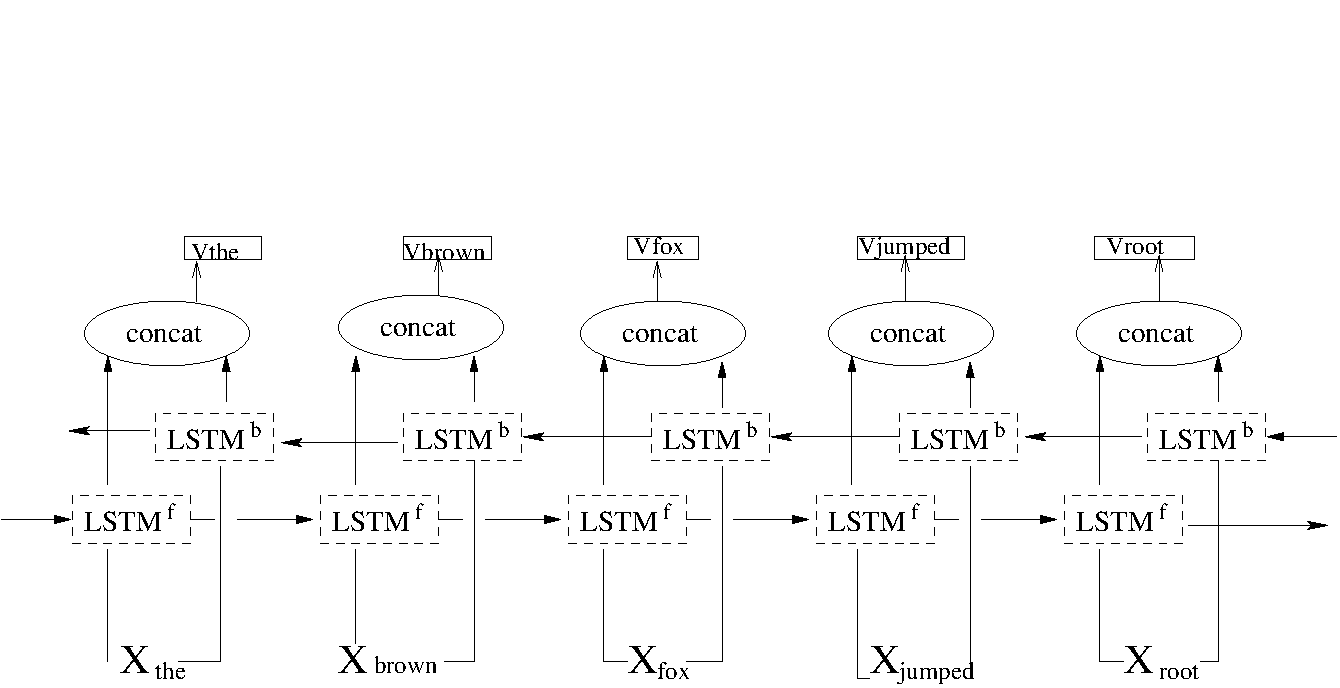
\includegraphics[scale=0.5]{images/comp0.pdf}
				\end{figure}
		}

		\only<2>{
				\begin{figure}
						\centering
						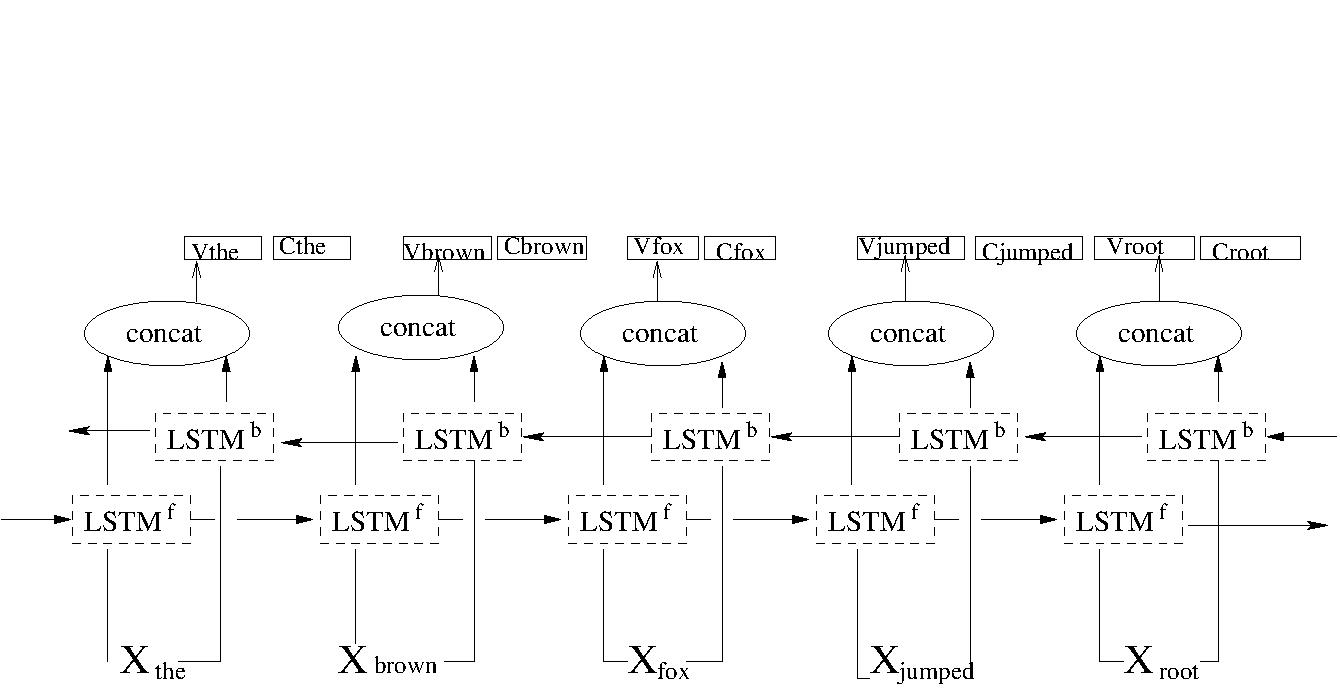
\includegraphics[scale=0.5]{images/comp1.pdf}
				\end{figure}
		}

		\only<3>{
				\begin{figure}
						\centering
						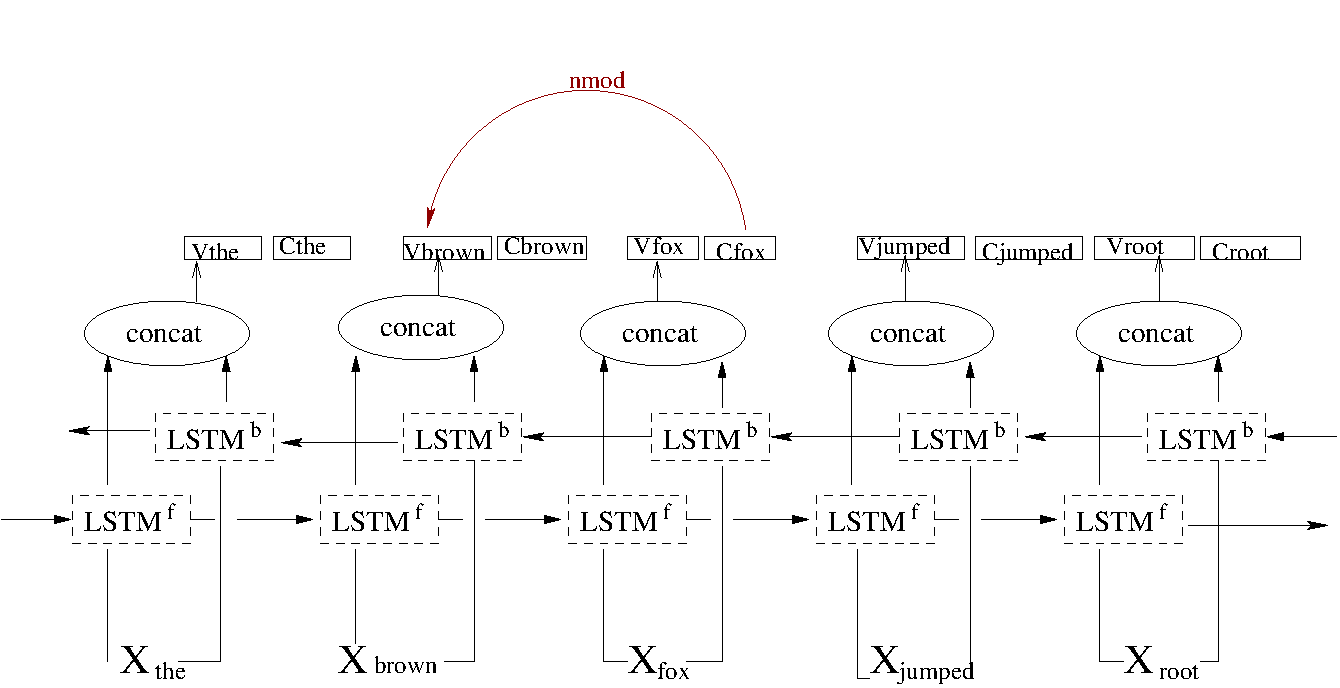
\includegraphics[scale=0.5]{images/comp2.pdf}
				\end{figure}
		}
		\only<4>{
				\begin{figure}
						\centering
						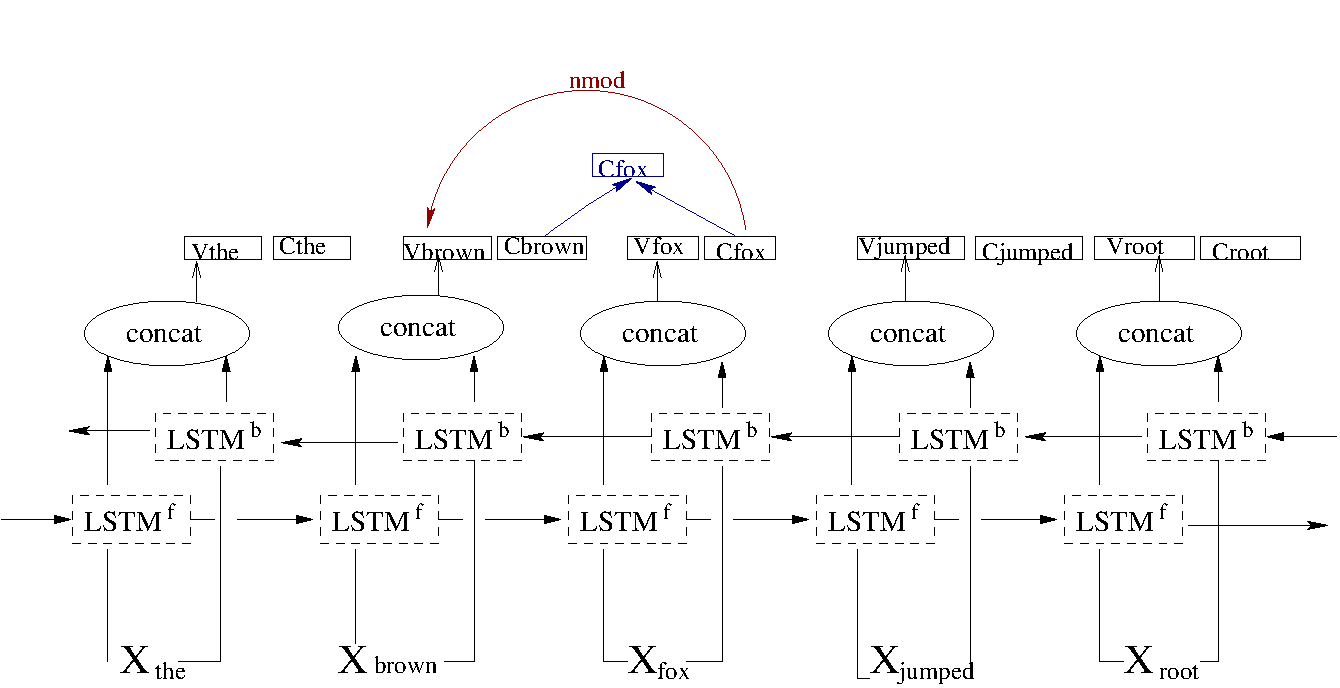
\includegraphics[scale=0.5]{images/comp3.pdf}
				\end{figure}
		}

		\only<5>{
				\begin{figure}
						\centering
						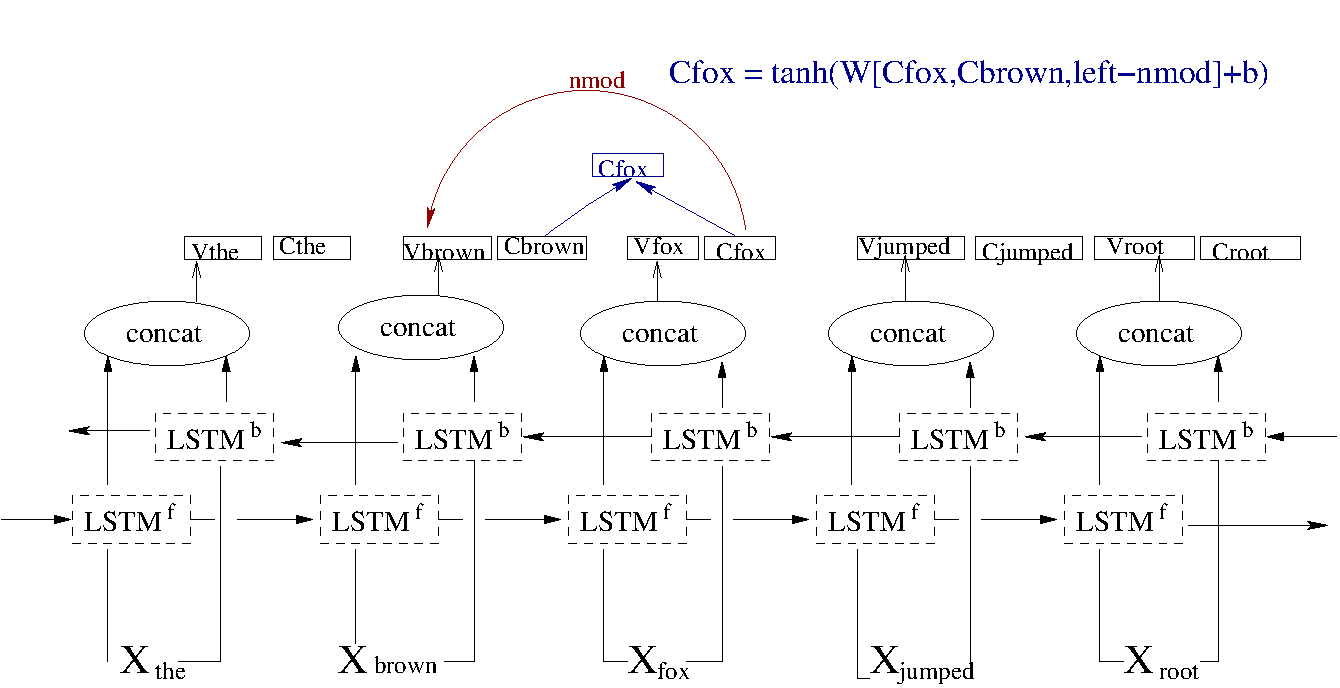
\includegraphics[scale=0.5]{images/comp4.pdf}
				\end{figure}
		}


		\only<6>{
				\begin{figure}
						\centering
						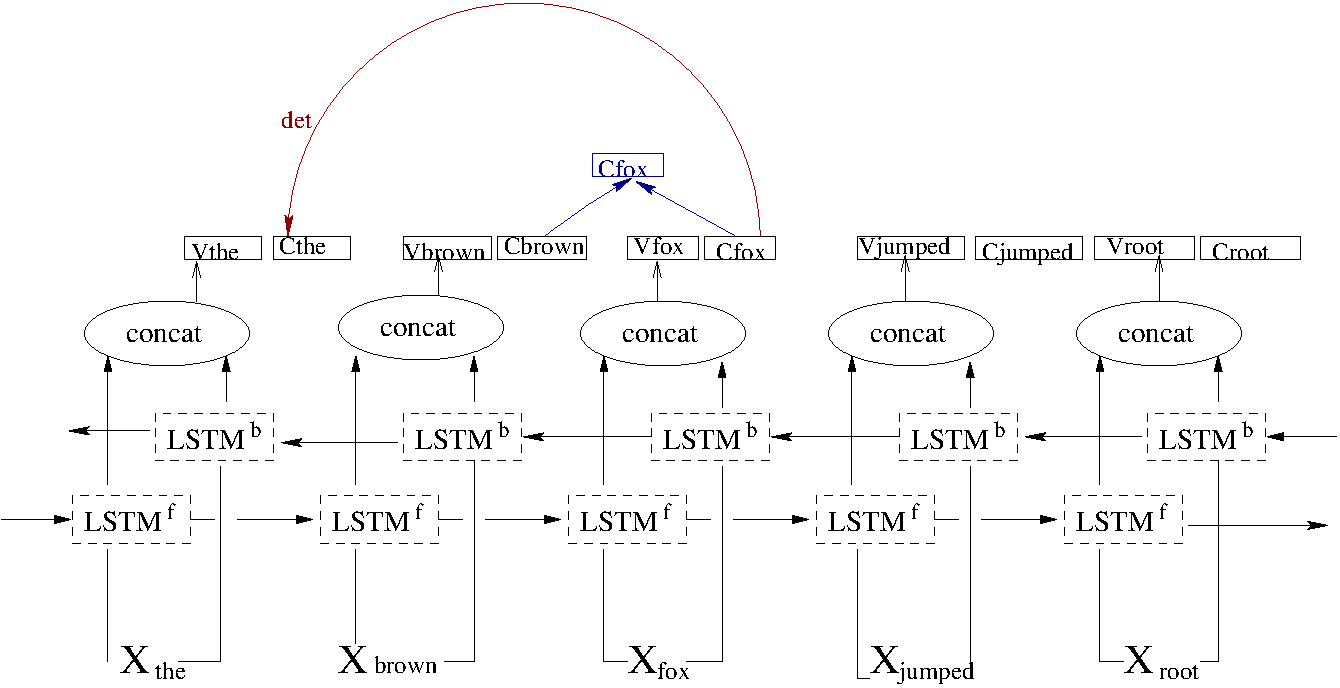
\includegraphics[scale=0.5]{images/comp5.pdf}
				\end{figure}
		}
		\only<7>{
				\begin{figure}
						\centering
						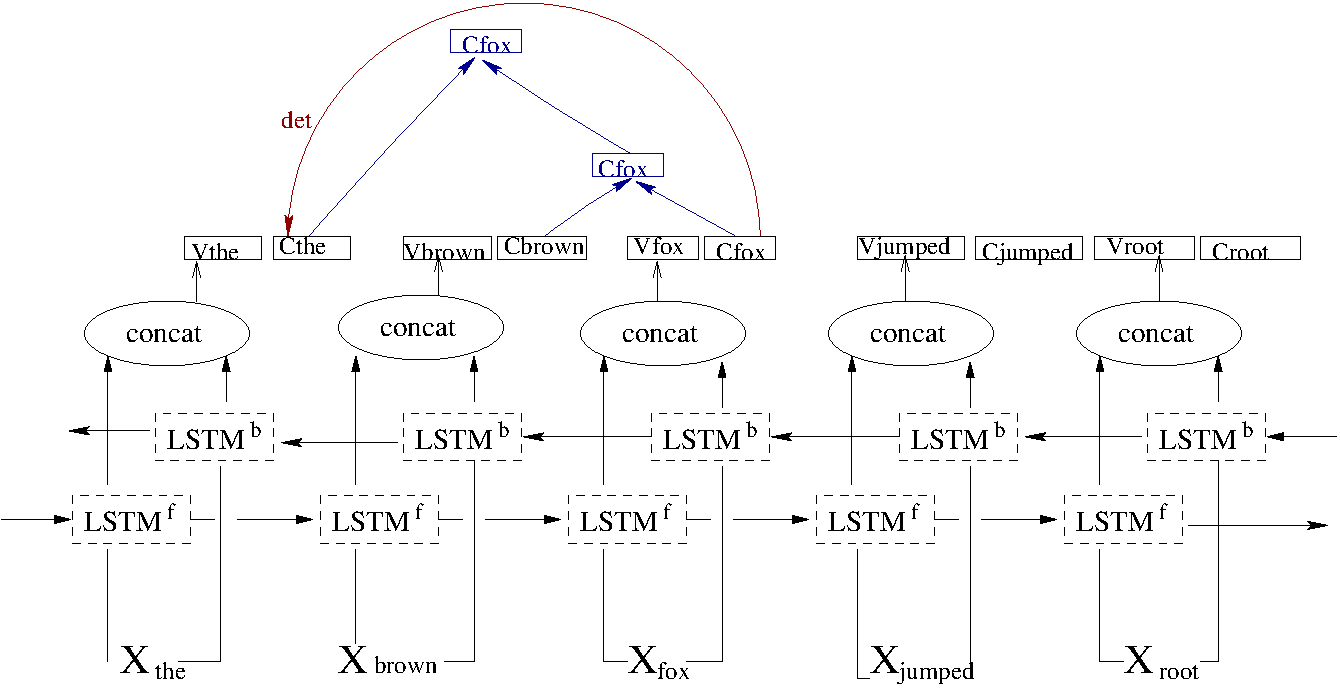
\includegraphics[scale=0.5]{images/comp6.pdf}
				\end{figure}
		}
		\vspace{1cm}
		\tiny{
		\textcite{delhoneux19recursive}
		}

\end{frame}

\subsection{Analyse en constituants : CKY et PCFG}

% TODO: Coavoux et Crabbé ?

\begin{frame}{Analyse en constituants}

	\centering
		\begin{forest}
		[S 
			[NP 
				[ I ] 
			]
			[VP 
				[V 
					[love]
				]
				[NP 
					[syntax] 
				] 
			]
		]
		\end{forest}

\end{frame}

% risk of top down: generate things that never match the input
% risk of bottom up: generate structure that cannot be part of a tree
\begin{frame}{CKY}
	Cocke–Younger–Kasami
	\begin{columns}
						\begin{column}{0.65\textwidth}

	\only<2>{
		%\vspace{-0.5cm}
\begin{table}[]
\begin{tabular}{lllllll}
{\color[HTML]{FFFFFF} NP} & {\color[HTML]{FFFFFF} S}     & {\color[HTML]{FFFFFF} }    & {\color[HTML]{FFFFFF} S}  & {\color[HTML]{FFFFFF} }  & {\color[HTML]{FFFFFF} }    & {\color[HTML]{FFFFFF} S}  \\
{\color[HTML]{FFFFFF} }   & {\color[HTML]{FFFFFF} \small{V, VP}} & {\color[HTML]{FFFFFF} }    & {\color[HTML]{FFFFFF} VP} & {\color[HTML]{FFFFFF} }  & {\color[HTML]{FFFFFF} }    & {\color[HTML]{FFFFFF} VP} \\
{\color[HTML]{FFFFFF} }   & {\color[HTML]{FFFFFF} }      & {\color[HTML]{FFFFFF} Det} & {\color[HTML]{FFFFFF} NP} & {\color[HTML]{FFFFFF} }  & {\color[HTML]{FFFFFF} }    & {\color[HTML]{FFFFFF} }   \\
{\color[HTML]{FFFFFF} }   & {\color[HTML]{FFFFFF} }      & {\color[HTML]{FFFFFF} }    & {\color[HTML]{FFFFFF} N}  & {\color[HTML]{FFFFFF} }  & {\color[HTML]{FFFFFF} }    & {\color[HTML]{FFFFFF} }   \\
{\color[HTML]{FFFFFF} }   & {\color[HTML]{FFFFFF} }      & {\color[HTML]{FFFFFF} }    & {\color[HTML]{FFFFFF} }   & {\color[HTML]{FFFFFF} P} & {\color[HTML]{FFFFFF} }    & {\color[HTML]{FFFFFF} PP} \\
{\color[HTML]{FFFFFF} }   & {\color[HTML]{FFFFFF} }      & {\color[HTML]{FFFFFF} }    & {\color[HTML]{FFFFFF} }   & {\color[HTML]{FFFFFF} }  & {\color[HTML]{FFFFFF} Det} & {\color[HTML]{FFFFFF} NP} \\
{\color[HTML]{FFFFFF} }   & {\color[HTML]{FFFFFF} }      & {\color[HTML]{FFFFFF} }    & {\color[HTML]{FFFFFF} }   & {\color[HTML]{FFFFFF} }  & {\color[HTML]{FFFFFF} }    & {\color[HTML]{FFFFFF} N}  \\
She                       & eats                         & a                          & fish                      & with                     & a                          & fork                     
\end{tabular}
\end{table}
	}
	\only<3>{
\begin{table}[]
\begin{tabular}{lllllll}
\hline
\multicolumn{1}{|l|}{{\color[HTML]{FFFFFF} NP}} & \multicolumn{1}{l|}{{\color[HTML]{FFFFFF} S}}     & \multicolumn{1}{l|}{}                           & \multicolumn{1}{l|}{{\color[HTML]{FFFFFF} S}}  & \multicolumn{1}{l|}{}                         & \multicolumn{1}{l|}{}                           & \multicolumn{1}{l|}{{\color[HTML]{FFFFFF} S}}  \\ \hline
\multicolumn{1}{l|}{}                           & \multicolumn{1}{l|}{{\color[HTML]{FFFFFF} \small{V,VP}}} & \multicolumn{1}{l|}{}                           & \multicolumn{1}{l|}{{\color[HTML]{FFFFFF} VP}} & \multicolumn{1}{l|}{}                         & \multicolumn{1}{l|}{}                           & \multicolumn{1}{l|}{{\color[HTML]{FFFFFF} VP}} \\ \cline{2-7} 
																								& \multicolumn{1}{l|}{}                             & \multicolumn{1}{l|}{{\color[HTML]{FFFFFF} Det}} & \multicolumn{1}{l|}{{\color[HTML]{FFFFFF} NP}} & \multicolumn{1}{l|}{}                         & \multicolumn{1}{l|}{}                           & \multicolumn{1}{l|}{}                          \\ \cline{3-7} 
																								&                                                   & \multicolumn{1}{l|}{}                           & \multicolumn{1}{l|}{{\color[HTML]{FFFFFF} N}}  & \multicolumn{1}{l|}{}                         & \multicolumn{1}{l|}{}                           & \multicolumn{1}{l|}{}                          \\ \cline{4-7} 
																								&                                                   &                                                 & \multicolumn{1}{l|}{}                          & \multicolumn{1}{l|}{{\color[HTML]{FFFFFF} P}} & \multicolumn{1}{l|}{}                           & \multicolumn{1}{l|}{{\color[HTML]{FFFFFF} PP}} \\ \cline{5-7} 
																								&                                                   &                                                 &                                                & \multicolumn{1}{l|}{}                         & \multicolumn{1}{l|}{{\color[HTML]{FFFFFF} Det}} & \multicolumn{1}{l|}{{\color[HTML]{FFFFFF} NP}} \\ \cline{6-7} 
																								&                                                   &                                                 &                                                &                                               & \multicolumn{1}{l|}{}                           & \multicolumn{1}{l|}{{\color[HTML]{FFFFFF} N}}  \\ \cline{7-7} 
She                                             & eats                                              & a                                               & fish                                           & with                                          & a                                               & fork                                          
\end{tabular}
\end{table}
	}
	\only<4>{
\begin{table}[]
\begin{tabular}{lllllll}
\hline
\multicolumn{1}{|l|}{NP} & \multicolumn{1}{l|}{{\color[HTML]{FFFFFF} S}}     & \multicolumn{1}{l|}{}                           & \multicolumn{1}{l|}{{\color[HTML]{FFFFFF} S}}  & \multicolumn{1}{l|}{}                         & \multicolumn{1}{l|}{}                           & \multicolumn{1}{l|}{{\color[HTML]{FFFFFF} S}}  \\ \hline
\multicolumn{1}{l|}{}    & \multicolumn{1}{l|}{{\color[HTML]{FFFFFF} \small{V,VP}}} & \multicolumn{1}{l|}{}                           & \multicolumn{1}{l|}{{\color[HTML]{FFFFFF} VP}} & \multicolumn{1}{l|}{}                         & \multicolumn{1}{l|}{}                           & \multicolumn{1}{l|}{{\color[HTML]{FFFFFF} VP}} \\ \cline{2-7} 
												 & \multicolumn{1}{l|}{}                             & \multicolumn{1}{l|}{{\color[HTML]{FFFFFF} Det}} & \multicolumn{1}{l|}{{\color[HTML]{FFFFFF} NP}} & \multicolumn{1}{l|}{}                         & \multicolumn{1}{l|}{}                           & \multicolumn{1}{l|}{}                          \\ \cline{3-7} 
												 &                                                   & \multicolumn{1}{l|}{}                           & \multicolumn{1}{l|}{{\color[HTML]{FFFFFF} N}}  & \multicolumn{1}{l|}{}                         & \multicolumn{1}{l|}{}                           & \multicolumn{1}{l|}{}                          \\ \cline{4-7} 
												 &                                                   &                                                 & \multicolumn{1}{l|}{}                          & \multicolumn{1}{l|}{{\color[HTML]{FFFFFF} P}} & \multicolumn{1}{l|}{}                           & \multicolumn{1}{l|}{{\color[HTML]{FFFFFF} PP}} \\ \cline{5-7} 
												 &                                                   &                                                 &                                                & \multicolumn{1}{l|}{}                         & \multicolumn{1}{l|}{{\color[HTML]{FFFFFF} Det}} & \multicolumn{1}{l|}{{\color[HTML]{FFFFFF} NP}} \\ \cline{6-7} 
												 &                                                   &                                                 &                                                &                                               & \multicolumn{1}{l|}{}                           & \multicolumn{1}{l|}{{\color[HTML]{FFFFFF} N}}  \\ \cline{7-7} 
She                      & eats                                              & a                                               & fish                                           & with                                          & a                                               & fork                                          
\end{tabular}
\end{table}
	}
	\only<5>{
\begin{table}[]
\begin{tabular}{lllllll}
\hline
\multicolumn{1}{|l|}{NP} & \multicolumn{1}{l|}{{\color[HTML]{FFFFFF} S}} & \multicolumn{1}{l|}{}                           & \multicolumn{1}{l|}{{\color[HTML]{FFFFFF} S}}  & \multicolumn{1}{l|}{}                         & \multicolumn{1}{l|}{}                           & \multicolumn{1}{l|}{{\color[HTML]{FFFFFF} S}}  \\ \hline
\multicolumn{1}{l|}{}    & \multicolumn{1}{l|}{\small{V,VP}}                    & \multicolumn{1}{l|}{}                           & \multicolumn{1}{l|}{{\color[HTML]{FFFFFF} VP}} & \multicolumn{1}{l|}{}                         & \multicolumn{1}{l|}{}                           & \multicolumn{1}{l|}{{\color[HTML]{FFFFFF} VP}} \\ \cline{2-7} 
												 & \multicolumn{1}{l|}{}                         & \multicolumn{1}{l|}{{\color[HTML]{FFFFFF} Det}} & \multicolumn{1}{l|}{{\color[HTML]{FFFFFF} NP}} & \multicolumn{1}{l|}{}                         & \multicolumn{1}{l|}{}                           & \multicolumn{1}{l|}{}                          \\ \cline{3-7} 
												 &                                               & \multicolumn{1}{l|}{}                           & \multicolumn{1}{l|}{{\color[HTML]{FFFFFF} N}}  & \multicolumn{1}{l|}{}                         & \multicolumn{1}{l|}{}                           & \multicolumn{1}{l|}{}                          \\ \cline{4-7} 
												 &                                               &                                                 & \multicolumn{1}{l|}{}                          & \multicolumn{1}{l|}{{\color[HTML]{FFFFFF} P}} & \multicolumn{1}{l|}{}                           & \multicolumn{1}{l|}{{\color[HTML]{FFFFFF} PP}} \\ \cline{5-7} 
												 &                                               &                                                 &                                                & \multicolumn{1}{l|}{}                         & \multicolumn{1}{l|}{{\color[HTML]{FFFFFF} Det}} & \multicolumn{1}{l|}{{\color[HTML]{FFFFFF} NP}} \\ \cline{6-7} 
												 &                                               &                                                 &                                                &                                               & \multicolumn{1}{l|}{}                           & \multicolumn{1}{l|}{{\color[HTML]{FFFFFF} N}}  \\ \cline{7-7} 
She                      & eats                                          & a                                               & fish                                           & with                                          & a                                               & fork                                          
\end{tabular}
\end{table}
	}
	\only<6>{
\begin{table}[]
\begin{tabular}{lllllll}
\hline
\multicolumn{1}{|l|}{NP} & \multicolumn{1}{l|}{{\color[HTML]{FFFFFF} S}} & \multicolumn{1}{l|}{}    & \multicolumn{1}{l|}{{\color[HTML]{FFFFFF} S}}  & \multicolumn{1}{l|}{}                         & \multicolumn{1}{l|}{}                           & \multicolumn{1}{l|}{{\color[HTML]{FFFFFF} S}}  \\ \hline
\multicolumn{1}{l|}{}    & \multicolumn{1}{l|}{\small{V,VP}}                    & \multicolumn{1}{l|}{}    & \multicolumn{1}{l|}{{\color[HTML]{FFFFFF} VP}} & \multicolumn{1}{l|}{}                         & \multicolumn{1}{l|}{}                           & \multicolumn{1}{l|}{{\color[HTML]{FFFFFF} VP}} \\ \cline{2-7} 
												 & \multicolumn{1}{l|}{}                         & \multicolumn{1}{l|}{Det} & \multicolumn{1}{l|}{{\color[HTML]{FFFFFF} NP}} & \multicolumn{1}{l|}{}                         & \multicolumn{1}{l|}{}                           & \multicolumn{1}{l|}{}                          \\ \cline{3-7} 
												 &                                               & \multicolumn{1}{l|}{}    & \multicolumn{1}{l|}{{\color[HTML]{FFFFFF} N}}  & \multicolumn{1}{l|}{}                         & \multicolumn{1}{l|}{}                           & \multicolumn{1}{l|}{}                          \\ \cline{4-7} 
												 &                                               &                          & \multicolumn{1}{l|}{}                          & \multicolumn{1}{l|}{{\color[HTML]{FFFFFF} P}} & \multicolumn{1}{l|}{}                           & \multicolumn{1}{l|}{{\color[HTML]{FFFFFF} PP}} \\ \cline{5-7} 
												 &                                               &                          &                                                & \multicolumn{1}{l|}{}                         & \multicolumn{1}{l|}{{\color[HTML]{FFFFFF} Det}} & \multicolumn{1}{l|}{{\color[HTML]{FFFFFF} NP}} \\ \cline{6-7} 
												 &                                               &                          &                                                &                                               & \multicolumn{1}{l|}{}                           & \multicolumn{1}{l|}{{\color[HTML]{FFFFFF} N}}  \\ \cline{7-7} 
She                      & eats                                          & a                        & fish                                           & with                                          & a                                               & fork                                          
\end{tabular}
\end{table}
	}
	\only<7>{
\begin{table}[]
\begin{tabular}{lllllll}
\hline
\multicolumn{1}{|l|}{NP} & \multicolumn{1}{l|}{{\color[HTML]{FFFFFF} S}} & \multicolumn{1}{l|}{}    & \multicolumn{1}{l|}{{\color[HTML]{FFFFFF} S}}  & \multicolumn{1}{l|}{}  & \multicolumn{1}{l|}{}    & \multicolumn{1}{l|}{{\color[HTML]{FFFFFF} S}}  \\ \hline
\multicolumn{1}{l|}{}    & \multicolumn{1}{l|}{\small{V,VP}}                    & \multicolumn{1}{l|}{}    & \multicolumn{1}{l|}{{\color[HTML]{FFFFFF} VP}} & \multicolumn{1}{l|}{}  & \multicolumn{1}{l|}{}    & \multicolumn{1}{l|}{{\color[HTML]{FFFFFF} VP}} \\ \cline{2-7} 
												 & \multicolumn{1}{l|}{}                         & \multicolumn{1}{l|}{Det} & \multicolumn{1}{l|}{{\color[HTML]{FFFFFF} NP}} & \multicolumn{1}{l|}{}  & \multicolumn{1}{l|}{}    & \multicolumn{1}{l|}{}                          \\ \cline{3-7} 
												 &                                               & \multicolumn{1}{l|}{}    & \multicolumn{1}{l|}{N}                         & \multicolumn{1}{l|}{}  & \multicolumn{1}{l|}{}    & \multicolumn{1}{l|}{}                          \\ \cline{4-7} 
												 &                                               &                          & \multicolumn{1}{l|}{}                          & \multicolumn{1}{l|}{P} & \multicolumn{1}{l|}{}    & \multicolumn{1}{l|}{{\color[HTML]{FFFFFF} PP}} \\ \cline{5-7} 
												 &                                               &                          &                                                & \multicolumn{1}{l|}{}  & \multicolumn{1}{l|}{Det} & \multicolumn{1}{l|}{{\color[HTML]{FFFFFF} NP}} \\ \cline{6-7} 
												 &                                               &                          &                                                &                        & \multicolumn{1}{l|}{}    & \multicolumn{1}{l|}{N}                         \\ \cline{7-7} 
She                      & eats                                          & a                        & fish                                           & with                   & a                        & fork                                          
\end{tabular}
\end{table}
	}
	\only<8>{
\begin{table}[]
\begin{tabular}{lllllll}
\hline
\multicolumn{1}{|l|}{\textcolor{blue}{NP}} & \multicolumn{1}{l|}{\textcolor{blue}{S}}     & \multicolumn{1}{l|}{}    & \multicolumn{1}{l|}{{\color[HTML]{FFFFFF} S}}  & \multicolumn{1}{l|}{}  & \multicolumn{1}{l|}{}    & \multicolumn{1}{l|}{{\color[HTML]{FFFFFF} S}}  \\ \hline
\multicolumn{1}{l|}{}    & \multicolumn{1}{l|}{\small{V,\textcolor{blue}{VP}}} & \multicolumn{1}{l|}{}    & \multicolumn{1}{l|}{{\color[HTML]{FFFFFF} VP}} & \multicolumn{1}{l|}{}  & \multicolumn{1}{l|}{}    & \multicolumn{1}{l|}{{\color[HTML]{FFFFFF} VP}} \\ \cline{2-7} 
												 & \multicolumn{1}{l|}{}      & \multicolumn{1}{l|}{Det} & \multicolumn{1}{l|}{{\color[HTML]{FFFFFF} NP}} & \multicolumn{1}{l|}{}  & \multicolumn{1}{l|}{}    & \multicolumn{1}{l|}{}                          \\ \cline{3-7} 
												 &                            & \multicolumn{1}{l|}{}    & \multicolumn{1}{l|}{N}                         & \multicolumn{1}{l|}{}  & \multicolumn{1}{l|}{}    & \multicolumn{1}{l|}{}                          \\ \cline{4-7} 
												 &                            &                          & \multicolumn{1}{l|}{}                          & \multicolumn{1}{l|}{P} & \multicolumn{1}{l|}{}    & \multicolumn{1}{l|}{{\color[HTML]{FFFFFF} PP}} \\ \cline{5-7} 
												 &                            &                          &                                                & \multicolumn{1}{l|}{}  & \multicolumn{1}{l|}{Det} & \multicolumn{1}{l|}{{\color[HTML]{FFFFFF} NP}} \\ \cline{6-7} 
												 &                            &                          &                                                &                        & \multicolumn{1}{l|}{}    & \multicolumn{1}{l|}{N}                         \\ \cline{7-7} 
She                      & eats                       & a                        & fish                                           & with                   & a                        & fork                                          
\end{tabular}
\end{table}
	}
	\only<9>{
\begin{table}[]
\begin{tabular}{lllllll}
\hline
\multicolumn{1}{|l|}{NP} & \multicolumn{1}{l|}{S}     & \multicolumn{1}{l|}{}    & \multicolumn{1}{l|}{{\color[HTML]{FFFFFF} S}}  & \multicolumn{1}{l|}{}  & \multicolumn{1}{l|}{}    & \multicolumn{1}{l|}{{\color[HTML]{FFFFFF} S}}  \\ \hline
\multicolumn{1}{l|}{}    & \multicolumn{1}{l|}{\small{V,VP}} & \multicolumn{1}{l|}{}    & \multicolumn{1}{l|}{{\color[HTML]{FFFFFF} VP}} & \multicolumn{1}{l|}{}  & \multicolumn{1}{l|}{}    & \multicolumn{1}{l|}{{\color[HTML]{FFFFFF} VP}} \\ \cline{2-7} 
& \multicolumn{1}{l|}{}      & \multicolumn{1}{l|}{\textcolor{blue}{Det}} & \multicolumn{1}{l|}{\textcolor{blue}{NP}}                        & \multicolumn{1}{l|}{}  & \multicolumn{1}{l|}{}    & \multicolumn{1}{l|}{}                          \\ \cline{3-7} 
&   & \multicolumn{1}{l|}{}    & \multicolumn{1}{l|}{\textcolor{blue}{N}}                         & \multicolumn{1}{l|}{}  & \multicolumn{1}{l|}{}    & \multicolumn{1}{l|}{}                          \\ \cline{4-7} 
												 &                            &                          & \multicolumn{1}{l|}{}                          & \multicolumn{1}{l|}{P} & \multicolumn{1}{l|}{}    & \multicolumn{1}{l|}{{\color[HTML]{FFFFFF} PP}} \\ \cline{5-7} 
												 &                            &                          &                                                & \multicolumn{1}{l|}{}  & \multicolumn{1}{l|}{Det} & \multicolumn{1}{l|}{{\color[HTML]{FFFFFF} NP}} \\ \cline{6-7} 
												 &                            &                          &                                                &                        & \multicolumn{1}{l|}{}    & \multicolumn{1}{l|}{N}                         \\ \cline{7-7} 
She                      & eats                       & a                        & fish                                           & with                   & a                        & fork                                          
\end{tabular}
\end{table}
	}
	\only<10>{
\begin{table}[]
\begin{tabular}{lllllll}
\hline
\multicolumn{1}{|l|}{NP} & \multicolumn{1}{l|}{S}     & \multicolumn{1}{l|}{}    & \multicolumn{1}{l|}{{\color[HTML]{FFFFFF} S}}  & \multicolumn{1}{l|}{}  & \multicolumn{1}{l|}{}    & \multicolumn{1}{l|}{{\color[HTML]{FFFFFF} S}}  \\ \hline
\multicolumn{1}{l|}{}    & \multicolumn{1}{l|}{\small{V,VP}} & \multicolumn{1}{l|}{}    & \multicolumn{1}{l|}{{\color[HTML]{FFFFFF} VP}} & \multicolumn{1}{l|}{}  & \multicolumn{1}{l|}{}    & \multicolumn{1}{l|}{{\color[HTML]{FFFFFF} VP}} \\ \cline{2-7} 
												 & \multicolumn{1}{l|}{}      & \multicolumn{1}{l|}{Det} & \multicolumn{1}{l|}{NP}                        & \multicolumn{1}{l|}{}  & \multicolumn{1}{l|}{}    & \multicolumn{1}{l|}{}                          \\ \cline{3-7} 
												 &                            & \multicolumn{1}{l|}{}    & \multicolumn{1}{l|}{N}                         & \multicolumn{1}{l|}{}  & \multicolumn{1}{l|}{}    & \multicolumn{1}{l|}{}                          \\ \cline{4-7} 
												 &                            &                          & \multicolumn{1}{l|}{}                          & \multicolumn{1}{l|}{P} & \multicolumn{1}{l|}{}    & \multicolumn{1}{l|}{{\color[HTML]{FFFFFF} PP}} \\ \cline{5-7} 
												 &                            &                          &                                                & \multicolumn{1}{l|}{}  & \multicolumn{1}{l|}{\textcolor{blue}{Det}} & \multicolumn{1}{l|}{\textcolor{blue}{NP}}                        \\ \cline{6-7} 
												 &                            &                          &                                                &                        & \multicolumn{1}{l|}{}    & \multicolumn{1}{l|}{\textcolor{blue}{N}}                         \\ \cline{7-7} 
She                      & eats                       & a                        & fish                                           & with                   & a                        & fork                                          
\end{tabular}
\end{table}
	}
	\only<11>{
\begin{table}[]
\begin{tabular}{lllllll}
\hline
\multicolumn{1}{|l|}{NP} & \multicolumn{1}{l|}{S}     & \multicolumn{1}{l|}{}    & \multicolumn{1}{l|}{{\color[HTML]{FFFFFF} S}} & \multicolumn{1}{l|}{}  & \multicolumn{1}{l|}{}    & \multicolumn{1}{l|}{{\color[HTML]{FFFFFF} S}}  \\ \hline
\multicolumn{1}{l|}{}    & \multicolumn{1}{l|}{\small{\textcolor{blue}{V},VP}} & \multicolumn{1}{l|}{}    & \multicolumn{1}{l|}{\textcolor{blue}{VP}}                       & \multicolumn{1}{l|}{}  & \multicolumn{1}{l|}{}    & \multicolumn{1}{l|}{{\color[HTML]{FFFFFF} VP}} \\ \cline{2-7} 
& \multicolumn{1}{l|}{}      & \multicolumn{1}{l|}{Det} & \multicolumn{1}{l|}{\textcolor{blue}{NP}}                       & \multicolumn{1}{l|}{}  & \multicolumn{1}{l|}{}    & \multicolumn{1}{l|}{}                          \\ \cline{3-7} 
												 &                            & \multicolumn{1}{l|}{}    & \multicolumn{1}{l|}{N}                        & \multicolumn{1}{l|}{}  & \multicolumn{1}{l|}{}    & \multicolumn{1}{l|}{}                          \\ \cline{4-7} 
												 &                            &                          & \multicolumn{1}{l|}{}                         & \multicolumn{1}{l|}{P} & \multicolumn{1}{l|}{}    & \multicolumn{1}{l|}{{\color[HTML]{FFFFFF} PP}} \\ \cline{5-7} 
												 &                            &                          &                                               & \multicolumn{1}{l|}{}  & \multicolumn{1}{l|}{Det} & \multicolumn{1}{l|}{NP}                        \\ \cline{6-7} 
												 &                            &                          &                                               &                        & \multicolumn{1}{l|}{}    & \multicolumn{1}{l|}{N}                         \\ \cline{7-7} 
She                      & eats                       & a                        & fish                                          & with                   & a                        & fork                                          
\end{tabular}
\end{table}
	}
	\only<12>{
\begin{table}[]
\begin{tabular}{lllllll}
\hline
\multicolumn{1}{|l|}{NP} & \multicolumn{1}{l|}{S}     & \multicolumn{1}{l|}{}    & \multicolumn{1}{l|}{{\color[HTML]{FFFFFF} S}} & \multicolumn{1}{l|}{}  & \multicolumn{1}{l|}{}    & \multicolumn{1}{l|}{{\color[HTML]{FFFFFF} S}}  \\ \hline
\multicolumn{1}{l|}{}    & \multicolumn{1}{l|}{\small{V,VP}} & \multicolumn{1}{l|}{}    & \multicolumn{1}{l|}{VP}                       & \multicolumn{1}{l|}{}  & \multicolumn{1}{l|}{}    & \multicolumn{1}{l|}{{\color[HTML]{FFFFFF} VP}} \\ \cline{2-7} 
												 & \multicolumn{1}{l|}{}      & \multicolumn{1}{l|}{Det} & \multicolumn{1}{l|}{NP}                       & \multicolumn{1}{l|}{}  & \multicolumn{1}{l|}{}    & \multicolumn{1}{l|}{}                          \\ \cline{3-7} 
												 &                            & \multicolumn{1}{l|}{}    & \multicolumn{1}{l|}{N}                        & \multicolumn{1}{l|}{}  & \multicolumn{1}{l|}{}    & \multicolumn{1}{l|}{}                          \\ \cline{4-7} 
												 &                            &                          & \multicolumn{1}{l|}{}                         & \multicolumn{1}{l|}{\textcolor{blue}{P}} & \multicolumn{1}{l|}{}    & \multicolumn{1}{l|}{\textcolor{blue}{PP}}                        \\ \cline{5-7} 
												 &                            &                          &                                               & \multicolumn{1}{l|}{}  & \multicolumn{1}{l|}{Det} & \multicolumn{1}{l|}{\textcolor{blue}{NP}}                        \\ \cline{6-7} 
												 &                            &                          &                                               &                        & \multicolumn{1}{l|}{}    & \multicolumn{1}{l|}{N}                         \\ \cline{7-7} 
She                      & eats                       & a                        & fish                                          & with                   & a                        & fork                                          
\end{tabular}
\end{table}
	}
	\only<13>{
\begin{table}[]
\begin{tabular}{lllllll}
\hline
\multicolumn{1}{|l|}{\textcolor{blue}{NP}} & \multicolumn{1}{l|}{S}     & \multicolumn{1}{l|}{}    & \multicolumn{1}{l|}{\textcolor{blue}{S}}  & \multicolumn{1}{l|}{}  & \multicolumn{1}{l|}{}    & \multicolumn{1}{l|}{{\color[HTML]{FFFFFF} S}}  \\ \hline
\multicolumn{1}{l|}{}    & \multicolumn{1}{l|}{\small{V,VP}} & \multicolumn{1}{l|}{}    & \multicolumn{1}{l|}{\textcolor{blue}{VP}} & \multicolumn{1}{l|}{}  & \multicolumn{1}{l|}{}    & \multicolumn{1}{l|}{{\color[HTML]{FFFFFF} VP}} \\ \cline{2-7} 
												 & \multicolumn{1}{l|}{}      & \multicolumn{1}{l|}{Det} & \multicolumn{1}{l|}{NP} & \multicolumn{1}{l|}{}  & \multicolumn{1}{l|}{}    & \multicolumn{1}{l|}{}                          \\ \cline{3-7} 
												 &                            & \multicolumn{1}{l|}{}    & \multicolumn{1}{l|}{N}  & \multicolumn{1}{l|}{}  & \multicolumn{1}{l|}{}    & \multicolumn{1}{l|}{}                          \\ \cline{4-7} 
												 &                            &                          & \multicolumn{1}{l|}{}   & \multicolumn{1}{l|}{P} & \multicolumn{1}{l|}{}    & \multicolumn{1}{l|}{PP}                        \\ \cline{5-7} 
												 &                            &                          &                         & \multicolumn{1}{l|}{}  & \multicolumn{1}{l|}{Det} & \multicolumn{1}{l|}{NP}                        \\ \cline{6-7} 
												 &                            &                          &                         &                        & \multicolumn{1}{l|}{}    & \multicolumn{1}{l|}{N}                         \\ \cline{7-7} 
She                      & eats                       & a                        & fish                    & with                   & a                        & fork                                          
\end{tabular}
\end{table}
	}
	\only<14>{
\begin{table}[]
\begin{tabular}{lllllll}
\hline
\multicolumn{1}{|l|}{NP} & \multicolumn{1}{l|}{S}     & \multicolumn{1}{l|}{}    & \multicolumn{1}{l|}{S}  & \multicolumn{1}{l|}{}  & \multicolumn{1}{l|}{}    & \multicolumn{1}{l|}{{\color[HTML]{FFFFFF} S}} \\ \hline
\multicolumn{1}{l|}{}    & \multicolumn{1}{l|}{\small{V,VP}} & \multicolumn{1}{l|}{}    & \multicolumn{1}{l|}{\textcolor{blue}{VP}} & \multicolumn{1}{l|}{}  & \multicolumn{1}{l|}{}    & \multicolumn{1}{l|}{\textcolor{blue}{VP}}                       \\ \cline{2-7} 
												 & \multicolumn{1}{l|}{}      & \multicolumn{1}{l|}{Det} & \multicolumn{1}{l|}{NP} & \multicolumn{1}{l|}{}  & \multicolumn{1}{l|}{}    & \multicolumn{1}{l|}{}                         \\ \cline{3-7} 
												 &                            & \multicolumn{1}{l|}{}    & \multicolumn{1}{l|}{N}  & \multicolumn{1}{l|}{}  & \multicolumn{1}{l|}{}    & \multicolumn{1}{l|}{}                         \\ \cline{4-7} 
												 &                            &                          & \multicolumn{1}{l|}{}   & \multicolumn{1}{l|}{P} & \multicolumn{1}{l|}{}    & \multicolumn{1}{l|}{\textcolor{blue}{PP}}                       \\ \cline{5-7} 
												 &                            &                          &                         & \multicolumn{1}{l|}{}  & \multicolumn{1}{l|}{Det} & \multicolumn{1}{l|}{NP}                       \\ \cline{6-7} 
												 &                            &                          &                         &                        & \multicolumn{1}{l|}{}    & \multicolumn{1}{l|}{N}                        \\ \cline{7-7} 
She                      & eats                       & a                        & fish                    & with                   & a                        & fork                                         
\end{tabular}
\end{table}
	}

	\only<15>{
\begin{table}[]
\begin{tabular}{lllllll}
\hline
\multicolumn{1}{|l|}{\textcolor{blue}{NP}} & \multicolumn{1}{l|}{S}     & \multicolumn{1}{l|}{}    & \multicolumn{1}{l|}{S}  & \multicolumn{1}{l|}{}  & \multicolumn{1}{l|}{}    & \multicolumn{1}{l|}{\textcolor{blue}{S}}  \\ \hline
\multicolumn{1}{l|}{}    & \multicolumn{1}{l|}{\small{V,VP}} & \multicolumn{1}{l|}{}    & \multicolumn{1}{l|}{VP} & \multicolumn{1}{l|}{}  & \multicolumn{1}{l|}{}    & \multicolumn{1}{l|}{\textcolor{blue}{VP}} \\ \cline{2-7} 
												 & \multicolumn{1}{l|}{}      & \multicolumn{1}{l|}{Det} & \multicolumn{1}{l|}{NP} & \multicolumn{1}{l|}{}  & \multicolumn{1}{l|}{}    & \multicolumn{1}{l|}{}   \\ \cline{3-7} 
												 &                            & \multicolumn{1}{l|}{}    & \multicolumn{1}{l|}{N}  & \multicolumn{1}{l|}{}  & \multicolumn{1}{l|}{}    & \multicolumn{1}{l|}{}   \\ \cline{4-7} 
												 &                            &                          & \multicolumn{1}{l|}{}   & \multicolumn{1}{l|}{P} & \multicolumn{1}{l|}{}    & \multicolumn{1}{l|}{PP} \\ \cline{5-7} 
												 &                            &                          &                         & \multicolumn{1}{l|}{}  & \multicolumn{1}{l|}{Det} & \multicolumn{1}{l|}{NP} \\ \cline{6-7} 
												 &                            &                          &                         &                        & \multicolumn{1}{l|}{}    & \multicolumn{1}{l|}{N}  \\ \cline{7-7} 
She                      & eats                       & a                        & fish                    & with                   & a                        & fork                   
\end{tabular}
\end{table}
	}

	\only<16>{
\begin{table}[]
\begin{tabular}{lllllll}
\hline
\multicolumn{1}{|l|}{NP} & \multicolumn{1}{l|}{S}     & \multicolumn{1}{l|}{}    & \multicolumn{1}{l|}{S}  & \multicolumn{1}{l|}{}  & \multicolumn{1}{l|}{}    & \multicolumn{1}{l|}{S}  \\ \hline
\multicolumn{1}{l|}{}    & \multicolumn{1}{l|}{\small{V,VP}} & \multicolumn{1}{l|}{}    & \multicolumn{1}{l|}{VP} & \multicolumn{1}{l|}{}  & \multicolumn{1}{l|}{}    & \multicolumn{1}{l|}{VP} \\ \cline{2-7} 
												 & \multicolumn{1}{l|}{}      & \multicolumn{1}{l|}{Det} & \multicolumn{1}{l|}{NP} & \multicolumn{1}{l|}{}  & \multicolumn{1}{l|}{}    & \multicolumn{1}{l|}{}   \\ \cline{3-7} 
												 &                            & \multicolumn{1}{l|}{}    & \multicolumn{1}{l|}{N}  & \multicolumn{1}{l|}{}  & \multicolumn{1}{l|}{}    & \multicolumn{1}{l|}{}   \\ \cline{4-7} 
												 &                            &                          & \multicolumn{1}{l|}{}   & \multicolumn{1}{l|}{P} & \multicolumn{1}{l|}{}    & \multicolumn{1}{l|}{PP} \\ \cline{5-7} 
												 &                            &                          &                         & \multicolumn{1}{l|}{}  & \multicolumn{1}{l|}{Det} & \multicolumn{1}{l|}{NP} \\ \cline{6-7} 
												 &                            &                          &                         &                        & \multicolumn{1}{l|}{}    & \multicolumn{1}{l|}{N}  \\ \cline{7-7} 
She                      & eats                       & a                        & fish                    & with                   & a                        & fork                   
\end{tabular}
\end{table}
	}

	\only<16>{
		\vspace{-0.52cm}
	}
\end{column}
\begin{column}{0.35\textwidth}
	%TODO: reduce space between columns
	\only<1-15>{
\begin{table}[]
\begin{tabular}{ll}
\multicolumn{2}{l}{Context-Free Grammar}  \\ \hline
S   &$\rightarrow$  NP VP \\
VP  &$\rightarrow$  VP PP \\
VP  &$\rightarrow$  V NP  \\
VP  &$\rightarrow$  eats  \\
PP  &$\rightarrow$  P NP  \\
NP  &$\rightarrow$  Det N \\
NP  &$\rightarrow$  She   \\
V   &$\rightarrow$  eats  \\
P   &$\rightarrow$  with  \\
N   &$\rightarrow$  fish  \\
N   &$\rightarrow$  fork  \\
Det &$\rightarrow$  a    
\end{tabular}
\end{table}
}
\only<16>{

	\tiny
		\begin{forest}
		[S 
			[NP 
				[ She ] 
			]
			[VP 
				[VP
					[V 
						[eats]
					]
					[NP
						[Det
							[a]
						]
						[N
							[fish]
						]
					]
				]
				[PP 
					[P
						[with]
					]
					[NP
						[Det
							[a]
						]
						[N
							[fork]
						]
					]
				] 
			]
		]
		\end{forest}

}
\end{column}
\end{columns}
\end{frame}

\begin{frame}{Chomsky Normal Form}
		\begin{overlayarea}{\textwidth}{0.6\textheight}
			\begin{block}{Constraints}
				\begin{itemize}
					\item<2-> Only binary rules
					\item<6-> No unit productions
				\end{itemize}
			\end{block}

\only<3>{
\begin{table}[]
\begin{tabular}{l|l}
original grammar                                                  & CNF                                                              \\ \cline{1-2}
{\color[HTML]{FFFFFF} }                                           & {\color[HTML]{FFFFFF} VP $\color[HTML]{FFFFFF}\rightarrow$ X PP}                     \\
\multirow{-2}{*}{{\color[HTML]{FFFFFF} VP $\color[HTML]{FFFFFF}\rightarrow$ V NP PP}} & {\color[HTML]{FFFFFF} X  $\color[HTML]{FFFFFF}\rightarrow$ V NP}                     \\
{\color[HTML]{FFFFFF} NP $\color[HTML]{FFFFFF}\rightarrow$ N}                         & {\color[HTML]{FFFFFF} }                                          \\
{\color[HTML]{FFFFFF} N $\color[HTML]{FFFFFF}\rightarrow$ fish}                       & \multirow{-2}{*}{{\color[HTML]{FFFFFF} NP $\color[HTML]{FFFFFF}\rightarrow$ fish}}  
\end{tabular}
\end{table}
}
\only<4>{
\begin{table}[]
\begin{tabular}{l|l}
original grammar                            & CNF                                                              \\ \cline{1-2}
																						& {\color[HTML]{FFFFFF} VP $\color[HTML]{FFFFFF}\rightarrow$ X PP}                     \\
\multirow{-2}{*}{VP $\rightarrow$ V NP PP}  & {\color[HTML]{FFFFFF} X  $\color[HTML]{FFFFFF}\rightarrow$ V NP}                     \\
{\color[HTML]{FFFFFF} NP $\color[HTML]{FFFFFF}\rightarrow$ N}   & {\color[HTML]{FFFFFF} }                                          \\
{\color[HTML]{FFFFFF} N $\color[HTML]{FFFFFF}\rightarrow$ fish} & \multirow{-2}{*}{{\color[HTML]{FFFFFF} NP $\color[HTML]{FFFFFF}\rightarrow$ fish}}  
\end{tabular}
\end{table}
}
\only<5-6>{
\begin{table}[]
\begin{tabular}{l|l}
original grammar                            & CNF                                                              \\ \cline{1-2}
																						& VP $\rightarrow$ X PP                                            \\
\multirow{-2}{*}{VP $\rightarrow$ V NP PP}  & X  $\rightarrow$ V NP                                            \\
{\color[HTML]{FFFFFF} NP $\color[HTML]{FFFFFF}\rightarrow$ N}   & {\color[HTML]{FFFFFF} }                                          \\
{\color[HTML]{FFFFFF} N $\color[HTML]{FFFFFF}\rightarrow$ fish} & \multirow{-2}{*}{{\color[HTML]{FFFFFF} NP $\color[HTML]{FFFFFF}\rightarrow$ fish}}  
\end{tabular}
\end{table}
}
\only<7>{
\begin{table}[]
\begin{tabular}{l|l}
original grammar                           & CNF                                                              \\ \cline{1-2}
																					 & VP $\rightarrow$ X PP                                            \\
\multirow{-2}{*}{VP $\rightarrow$ V NP PP} & X  $\rightarrow$ V NP                                            \\
NP $\rightarrow$ N                         & {\color[HTML]{FFFFFF} }                                          \\
N $\rightarrow$ fish                       & \multirow{-2}{*}{{\color[HTML]{FFFFFF} NP $\color[HTML]{FFFFFF}\rightarrow$ fish}}  
\end{tabular}
\end{table}
}
			\only<8>{
\begin{table}[]
\begin{tabular}{l|l}
original grammar                          & CNF                                      \\ \cline{1-2}
\multirow{2}{*}{VP $\rightarrow$ V NP PP} & VP $\rightarrow$ X PP                    \\
																					& X  $\rightarrow$ V NP                    \\
NP $\rightarrow$ N                        & \multirow{2}{*}{NP $\rightarrow$ fish}   \\
N $\rightarrow$ fish                      &                                         
\end{tabular}
\end{table}
}


\end{overlayarea}
\end{frame}

\begin{frame}{Probabilistic Context Free Grammars (PCFG)}
		\begin{overlayarea}{\textwidth}{0.8\textheight}
	\only<1>{
\begin{table}[]
\begin{tabular}{r|ll}
	\multicolumn{3}{l}{\textcolor{white}{Probabilistic} Context-Free Grammar}  \\ \hline
	\textcolor{white}{1} & S   &$\rightarrow$  NP VP \\
	\textcolor{white}{0.5} & VP  &$\rightarrow$  VP PP \\
	\textcolor{white}{0.4} & VP  &$\rightarrow$  V NP  \\
	\textcolor{white}{0.1} & VP  &$\rightarrow$  eats  \\
	\textcolor{white}{1} & PP  &$\rightarrow$  P NP  \\
	\textcolor{white}{0.8} & NP  &$\rightarrow$  Det N \\
	\textcolor{white}{0.2} & NP  &$\rightarrow$  She   \\
	\textcolor{white}{1} & V   &$\rightarrow$  eats  \\
	\textcolor{white}{1} & P   &$\rightarrow$  with  \\
	\textcolor{white}{0.5} & N   &$\rightarrow$  fish  \\
	\textcolor{white}{0.5} & N   &$\rightarrow$  fork  \\
	\textcolor{white}{1} & Det &$\rightarrow$  a    
\end{tabular}
\end{table}
	}

	\only<2>{
\begin{table}[]
\begin{tabular}{r|ll}
\multicolumn{3}{l}{Probabilistic Context-Free Grammar}  \\ \hline
1 & S   &$\rightarrow$  NP VP \\
0.5 & VP  &$\rightarrow$  VP PP \\
0.4 & VP  &$\rightarrow$  V NP  \\
0.1 & VP  &$\rightarrow$  eats  \\
1 & PP  &$\rightarrow$  P NP  \\
0.8 & NP  &$\rightarrow$  Det N \\
0.2 & NP  &$\rightarrow$  She   \\
1 & V   &$\rightarrow$  eats  \\
1 & P   &$\rightarrow$  with  \\
0.5 & N   &$\rightarrow$  fish  \\
0.5 & N   &$\rightarrow$  fork  \\
1 & Det &$\rightarrow$  a    
\end{tabular}
\end{table}
}
\end{overlayarea}
\end{frame}

% \begin{frame}{Analyse en constituants neuronale}
% 	\begin{figure}
% 		\centering
% 		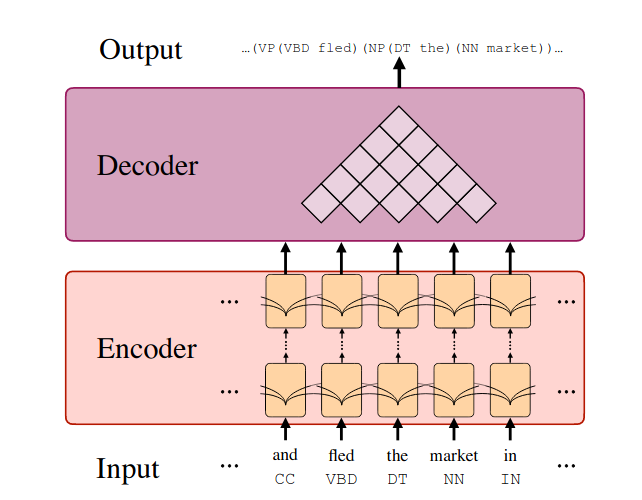
\includegraphics[scale=0.4]{images/const_parser}
% 	\end{figure}

% 	\vfill
% 	\tiny{\textcite{kitaev-klein-2018-constituency}}
% \end{frame}

\begin{frame}{Analyse en constituants neuronale}
	\begin{figure}
		\centering
		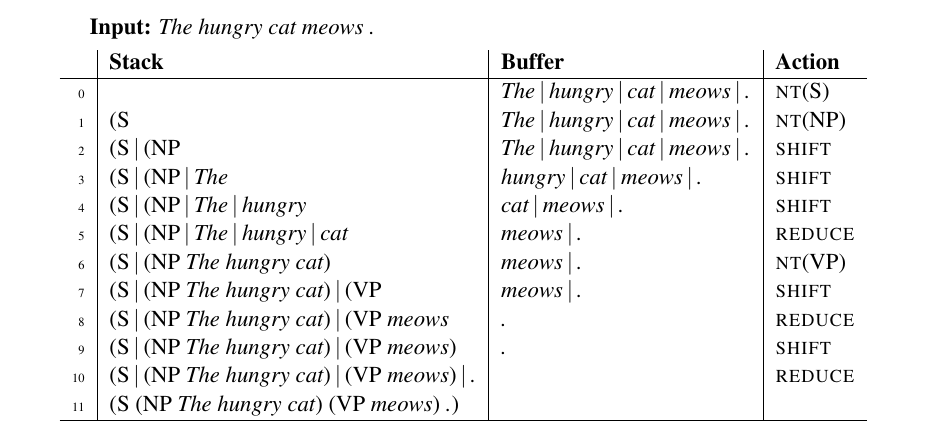
\includegraphics[scale=0.5]{images/rnng}
	\end{figure}

	\vfill
	\tiny{\textcite{dyer-etal-2016-recurrent}}
\end{frame}

\begin{frame}{Parsing génératif}
	\begin{figure}
		\centering
		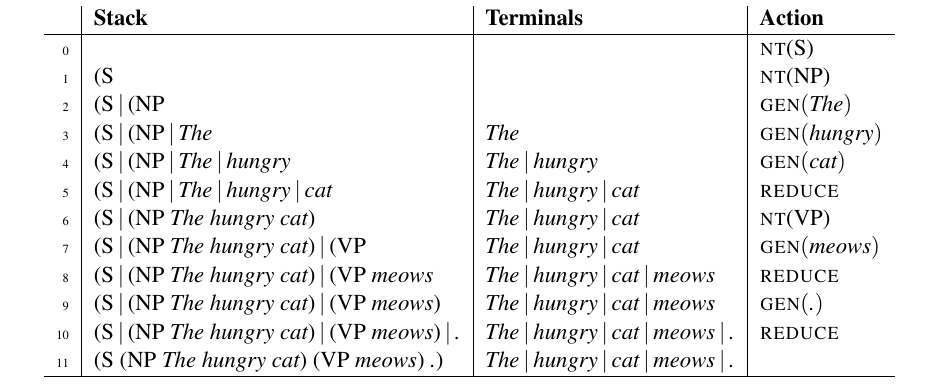
\includegraphics[scale=0.5]{images/rnng_states.png}
	\end{figure}

	\vfill
	\tiny{\textcite{dyer-etal-2016-recurrent}}
\end{frame}

\begin{frame}{En résumé}
	\begin{block}{}
		\begin{itemize}
			\item Syntax: dependency and constituency
			\item Dependency parsing: transition-based and graph-based
			\item Models: Recurrent and recursive neural networks
			\item Constituency parsing: CKY and PCFGs
		\end{itemize}
	\end{block}
\end{frame}

% \begin{frame}{Thanks!}
% 		\begin{center}
% 			\begin{dependency}[theme=simple,red]
% 				\begin{deptext}[column sep=1em]
% 					Do \& you \& have \& questions \&?  \\
% 				\end{deptext}
% 				\depedge{3}{1}{}
% 				\depedge{3}{2}{}
% 				\depedge{3}{4}{}
% 				\depedge{3}{5}{}
% 				\deproot{3}{}
% 			\end{dependency}
% 		\end{center}
% \end{frame}

%\begin{frame}{Additional material: optional exercises}
%  \begin{itemize}
%    \item Annotation: download a treebank in a language you are familiar with here: \url{https://universaldependencies.org/}, copy the annotation of simple sentences to a new file, replace all column 7 values (head) by an underscore. Then import the file to \url{https://maryszmary.github.io/ud-annotatrix/standalone/annotator.html#} and see if you can annotate it following the UD guidelines.
%    \item Transition-based exercise: Go to zzi.sh, type tnf57484 and follow the instructions.
%    \item CKY: go to \url{https://www.xarg.org/tools/cyk-algorithm/} and work out the example. You can verify your answers by clicking on step. You can modify the grammar and sequence to parse to try more exercises.
%    %\item Google for more or write me an email.
%  \end{itemize}
%\end{frame}

%  █████  ██████  ██████  ███████ ███    ██ ██████  ██ ██   ██
% ██   ██ ██   ██ ██   ██ ██      ████   ██ ██   ██ ██  ██ ██
% ███████ ██████  ██████  █████   ██ ██  ██ ██   ██ ██   ███
% ██   ██ ██      ██      ██      ██  ██ ██ ██   ██ ██  ██ ██
% ██   ██ ██      ██      ███████ ██   ████ ██████  ██ ██   ██

\hypersetup{bookmarksdepth=0}  % Don't create the bookmark for the Appendix part
\appendix
\hypersetup{bookmarksdepth=2}
\bookmarksetup{startatroot}
\section{Appendix}

\begin{frame}{Remerciements}
	Tous mes remerciements à Miryam de Lhoneux, autrice de la première version de ce cours et de ses diapositives en anglais.

	\shorturl{mdelhoneux.github.io}
\end{frame}


\pdfbookmark[3]{References}{references}
\begin{frame}[allowframebreaks]{References}
	\printbibliography[heading=none]
\end{frame}

\pdfbookmark[3]{Licence}{licence}
\begin{frame}{Licence}
	\begin{center}
		{\huge \ccby}
		\vfill
		This document is distributed under the terms of the Creative Commons Attribution 4.0 International Licence (CC BY 4.0) (\shorturl{creativecommons.org/licenses/by/4.0})

		\vfill
		© 2021, Loïc Grobol <\shorturl[mailto][:]{loic.grobol@gmail.com}>

		\shorturl[http]{http://www.llf.cnrs.fr/fr/Gens/Grobol}
	\end{center}
\end{frame}


\end{document} 
